\PassOptionsToPackage{dvipsnames}{xcolor}
\documentclass{llncs}


\usepackage{amsmath,amsfonts,amssymb}
\usepackage{adjustbox}
\usepackage{tikz}
\usepackage{tikzscale}
\usepackage{multirow}
%\usepackage[dvipsnames]{xcolor}
\usepackage{rotating}
\usepackage{tabularx}
\usepackage{booktabs}
\usepackage{arydshln}
\usepackage[noend]{algpseudocode}
\usepackage[backref,hidelinks]{hyperref}
\usepackage[capitalise]{cleveref}
\usetikzlibrary{cd}

\newcommand\Tstrut{\rule{0pt}{2.6ex}}         % = `top' strut
\newcommand\Bstrut{\rule[-0.9ex]{0pt}{0pt}}   % = `bottom' strut

\newcolumntype{b}{X}
\newcolumntype{s}{>{\hsize=.5\hsize}X}
\newcolumntype{B}{>{\hsize=1.3\hsize}X}

%\newcolumntype{u}{X}
%\newcolumntype{v}{>{\hsize=.4\hsize}X}
%\newcolumntype{w}{>{\hsize=.85\hsize}X}


\newcommand{\com}{\mathsf{com}}
\newcommand{\chall}{\mathsf{chall}}
\newcommand{\resp}{\mathsf{resp}}
\newcommand{\Com}{\ensuremath{\mathsf{C}}}

\newcommand{\Z}{\ensuremath{\mathbb{Z}}}
\newcommand{\N}{\ensuremath{\mathbb{N}}}
\newcommand{\F}{\ensuremath{\mathbb{F}}}
\newcommand{\Fbar}{\ensuremath{\overline{\mathbb{F}}}}
\newcommand{\Q}{\ensuremath{\mathbb{Q}}}
\newcommand{\OO}{\ensuremath{\mathcal{O}}}
\newcommand{\PO}{\ensuremath{O}}
\newcommand{\R}[1][]{\ensuremath{\mathcal{R}_{\mathrm{#1}}}}

\newcommand{\End}{\text{End}}
\newcommand{\comment}[1]{{\color{gray}#1}}
\newcommand{\develop}[1]{{\color{blue}#1}}
\newcommand{\CP}[1]{\comment{Christophe: #1}}
\newcommand{\LDF}[1]{\comment{Luca: #1}}
\newcommand{\SG}[1]{\comment{Steven: #1}}
\newcommand{\WB}[1]{\comment{Ward: #1}}

\renewcommand{\a}{\mathfrak{a}}
\renewcommand{\b}{\mathfrak{b}}
\renewcommand{\c}{\mathfrak{c}}

\newcommand{\CC}{\mathcal{C}}
\newcommand{\VV}{\mathcal{V}}
\newcommand{\PP}{\mathcal{P}}
\newcommand{\HH}{\mathcal{H}}
\newcommand{\Sim}{\mathcal{S}}
\newcommand{\Rela}{\mathcal{R}}
\newcommand{\A}{\mathcal{A}}

\newcommand{\pk}{\mathsf{pk}}
\newcommand{\sk}{\mathsf{sk}}
\newcommand{\Gen}{\mathsf{Gen}}
\newcommand{\KeyGen}{\mathsf{KeyGen}}
\newcommand{\Sign}{\mathsf{Sign}}
\newcommand{\Verify}{\mathsf{Verify}}
\newcommand{\EUFCMA}{\mathsf{EUF\text{-}CMA}}
\newcommand{\Field}{\mathbb{F}}
\newcommand{\fl}{\mathfrak{l}}
\newcommand{\fg}{\mathfrak{g}}
\newcommand{\cl}{\text{cl}}
\newcommand{\Ell}{\mathcal{E}\ell\ell}
\newcommand{\bx}{\mathbf{x}}
\newcommand{\bb}{\mathbf{b}}
\newcommand{\br}{\mathbf{r}}
%\newcommand{\Ell}{{\mathcal{ELL}}}
%\newcommand{\cl}{{\text{Cl}}}

\renewcommand{\star}{*}

% I (Ward) put this here, because I find it much more readable, and we don't really have to worry about a page limit. Feel free to remove if you don't agree.
\setlength\parindent{0pt}
\setlength{\parskip}{1em}

\begin{document}
\pagestyle{plain}

\title{Proving knowledge of isogenies -- A survey}


\author{Ward Beullens\inst{1} \and Luca De Feo\inst{1} \and Steven D. Galbraith\inst{2} \and Christophe Petit\inst{3}}

\institute{IBM Research Europe, Zürich, Switzerland.
\email{wbe@zurich.ibm.com, des.cod.crypt.2022@defeo.lu}
\and
University of Auckland, New Zealand. \email{s.galbraith@auckland.ac.nz}
% ORCID 0000-0001-7114-8377
\and
University of Birmingham and Université libre de Bruxelles.  \email{christophe.f.petit@gmail.com}}

\maketitle


\begin{abstract}
Isogeny-based cryptography is an active area of research in post-quantum public key cryptography.
The problem of proving knowledge of an isogeny is a natural problem that has several applications in isogeny-based cryptography, such as to allow users to demonstrate that they are behaving honestly in a protocol.
It is also related to isogeny-based digital signatures.
Over the last few years there have been a number of advances in this area, but there are still many open problems.
The aim of this paper is to give an overview of the topic, and to highlight some open problems and directions for future research.
\end{abstract}

\keywords{isogeny, post-quantum cryptography, zero-knowledge}

%\tableofcontents

\section{Introduction}\label{sec1}


Let $E_0$ and $E_1$ be elliptic curves.
An isogeny is a map $\phi : E_0 \to E_1$ that is a morphism in the sense of algebraic geometry (it maps points on the curve $E_0$ to points on the curve $E_1$) and also a morphism in the sense of groups (a group homomorphism).
If there is an isogeny $\phi : E_0 \to E_1$ then there is also an isogeny $\hat{\phi} : E_1 \to E_0$, called the dual isogeny.
Two curves are called isogenous if there is an isogeny between them.
Given two isogenous elliptic curves $E_0$ and $E_1$ over a finite field $\F_q$ it is believed to be computationally hard (even for quantum computers) to compute an isogeny between them.
A natural problem is therefore for an entity to prove that they know an isogeny $\phi : E_0 \to E_1$ between two public elliptic curves $E_0$ and $E_1$ without revealing the isogeny.

Tate's isogeny theorem (due to Deuring in the elliptic curve case) states that two elliptic curves $E_0$ and $E_1$ over a finite field $\F_q$ are isogenous over $\F_q$ if $\#E_0( \F_q ) = \#E_1(\F_q)$. Since there are  polynomial time algorithms to compute $\#E_0( \F_q )$ it follows that one can determine in polynomial time whether two curves are isogenous. However, this is not the end of the story, since for cryptographic applications one often wants to prove knowledge of an isogeny between $E_0$ and $E_1$, possibly with some additional restrictions, e.g., on its degree.

Indeed, there are (at least) six NP-relations that have been studied in the setting of isogeny-based cryptography.
These relations are defined as sets of pairs $(x,w)$ where $x$ is the \emph{statement} and $w$ is a \emph{witness}.
Each relation defines a \emph{language} $L = \{ x : \exists w, (x,w) \in \R \}$.
For simplicity we define the relations for a fixed field $\F_q$.
In each of the relations below, $E_0,E_1$ denote elliptic curves and $\phi$ denotes an isogeny (the witness), all defined over $\F_q$.
We implicitly assume that witnesses can be represented in polynomial space and evaluated in polynomial time.
\begin{align*}
    \R[triv] &= \bigl\{ \bigl((E_0, E_1), \bot \bigr) \,\big\vert\, \#E_0( \F_q ) = \#E_1(\F_q), \text{ so } E_0, E_1 \text{ isogenous over } \F_q \bigr\};\\
    \R[isog]  &= \bigl\{ \bigl((E_0, E_1),\phi \bigr) \,\big\vert\, \phi : E_0 \to E_1 \text{ is an arbitrary isogeny}\bigr\};\\
    \R[deg]   &= \bigl\{ \bigl((E_0, E_1, d), \phi\bigr) \,\big\vert\, \phi : E_0 \to E_1 \text{ is an isogeny of degree } d \bigr\};\\
    \R[SIDH]  &= \bigl\{ \bigl((E_0, E_1, d, D, P_0, Q_0, P_1, Q_1 ),\phi \bigr) \\
              &\qquad \big\vert\, \phi : E_0 \to E_1 \text{ is an isogeny of degree } d \\
              &\qquad \text{ and } P_1 = \phi(P_0), Q_1 = \phi(Q_0) \\
              &\qquad \text{ where } E_0[D] = \langle P_0, Q_0\rangle  \text{ and } \gcd(D,d) = 1 \bigr\} ;\\
    \R[M-SIDH]&= \bigl\{ \bigl((E_0, E_1, d, D, P_0, Q_0, P_1, Q_1 ),\phi \bigr) \\
              &\qquad \big\vert\, \phi : E_0 \to E_1 \text{ is an isogeny of degree } d \\
              &\qquad \text{ and } P_1 = \lambda\phi(P_0), Q_1 = \lambda\phi(Q_0) \\
              &\qquad \text{ and } \lambda^2 = 1 \mod D \\
              &\qquad \text{ where } E_0[D] = \langle P_0, Q_0\rangle  \text{ and } \gcd(D,d) = 1 \bigr\} ;\\
    \R[CSIDH] &= \text{See Definition~\ref{defn:R-CSIDH} in Section~\ref{sec:CSIDH}.}
\end{align*}
%For precise details of \R[CSIDH] see Definition~\ref{defn:R-CSIDH} in Section~\ref{sec:CSIDH}. \CP{$E$ not defined. Maybe write $\R[CSIDH]  = \bigl\{ \bigl((E_0, E_1),\phi \bigr) \,\big\vert\, E_0,E_1,\phi \text{ all defined over } \mathbb{F}_p\bigr\}$} \LDF{\R[CSIDH] looks an awful lot like \R[isog]: the fact the isogeny is defined over the base field is anyway implicit in all relations.}

As we just said, the language $(E_0,E_1)$ of isogenous curves can be decided in polynomial time, hence the trivial witness $\bot$ in \R[triv].
%\LDF{Alternatively, $N = \# E_0 = \# E_1$ could be the witness. Unsure about what's easier to parse for the reader.}
The relations \R[isog] and \R[deg] are the main focus of this survey.
These two relations are believed to be hard in the sense that there is no efficient algorithm known to compute a witness when given an arbitrary element of the language. For $\R[deg]$ even deciding the language is usually hard (depending on $d$).
%We also introduce the relation \R[CSIDH]; see Section~\ref{sec:CSIDH}.

The relation \R[SIDH] is no longer relevant due to the devastating attacks discovered in 2022 by Castryck and Decru~\cite{CD22}, Maino and Martindale~\cite{MM22} and Robert~\cite{Rob22}. However, we briefly mention SIDH in a few places for historical reasons, and since some aspects of it are used to build protocols for the other relations. The relation \R[M-SIDH] is equivalent to \R[SIDH] when $D$ is a power of a prime, indeed in this case there are only two or four possibilities for the square root of unity $\lambda$. When $D$ contains many prime factors, however \R[M-SIDH] is believed to be harder than \R[SIDH], and has been proposed as an alternative foundation for an SIDH-like key exchange~\cite{cryptoeprint:2023/013}.





\subsubsection{Motivation.}
%
The main motivation for zero-knowledge proofs of knowledge of an isogeny is in ensuring that public keys in a system are correctly formed and that the owner of a public key does know the corresponding private key. Some systems require such ``proof of possession'' checks when a user registers their public key, to prevent malicious behaviour such as a user registering another user's public key as their own. For discussion see Section 4.3 of the X.509 RFC~\cite{X509}, and \cite{BFPW07}. 


Zero-knowledge proofs are also useful to defeat active attacks in cryptographic protocols. A passively secure protocol can indeed be turned into an actively secure one by requiring all parties to accompany each message they send with a zero-knowledge proof that the message has been generated correctly as specified by the protocol.
%
A recent example of this is given in ~\cite{cryptoeprint:2022/1469}.
An earlier example of this (now obsolete) is that the SIDH protocol~\cite{DFJP14} is vulnerable to the \emph{GPST attack}~\cite{GPST16}, in which an attacker deviates from the protocol to progressively learn the secret key of its victim. 
%We give the details in Section~\ref{sec:SIDH}. 
In the key encapsulation mechanism SIKE based on SIDH~\cite{sike2017}, this attack was defeated using a variant of the Fujisaki-Okamoto transform, but this involved generating and communicating ephemeral keys. In contrast, a solution based on a non-interactive proof of knowledge would have allowed static keys and non interactive key exchange.



Proofs of knowledge have other applications as well, most notably they give digital signature schemes through the Fiat-Shamir transform and variants. 
%
The RSA and ECDSA signature schemes currently in use are based on the hardness of integer factoring and the elliptic curve discrete logarithm problem, which will be solved efficiently when large scale quantum computers are available.
It is important to develop new signature schemes with post-quantum security.
%
Isogeny-based cryptography is believed to resist quantum computers, hence it is a natural and important question to build efficient digital signatures from isogeny problems. A natural way to build those signatures is to first develop zero-knowledge proofs of knowledge for isogeny relations.









\subsubsection{A simple approach that does not work.}\label{sec:simple}


               
To introduce some of the challenges in developing zero-knowledge proofs for the relations above, we first describe a simple idea for the second relation, namely to adapt the classic \emph{Goldreich, Micali, Wigderson (GMW)} zero-knowledge proof of graph isomorphism~\cite{GMW} (see Section~\ref{sec:GMW}), and we explain why a straightforward adaptation does not work. 

Let $\phi : E_0 \to E_1$ be an $\F_q$-isogeny, which is the witness known to the prover.
The natural idea is to choose a random isogeny $\psi : E_1 \to E_2$.
Due to the expansion properties of isogeny graphs (discussed in Section~\ref{sec:isog-graph}), if $\psi$ corresponds to a long enough walk in the graph then $E_2$ is uniformly distributed in the set of supersingular curves.
Set the commitment to be $E_2$.
The challenger sends a challenge $\chall \in \{0,1\}$.
When $\chall = 0$ the prover responds with a description of $\psi$, and when $\chall=1$ the prover responds with $\rho := \psi \circ \phi$.
The verifier checks that the response is an isogeny from $E_{1-\chall}$ to $E_2$, and accepts if this is the case.

One might think this could be zero knowledge, since $E_2$ is distributed uniformly and so can be simulated without knowing the witness.
But the problem is that $\psi \circ \phi$ can leak the witness $\phi$.
The details depend on how the isogeny $\psi \circ \phi$ is represented (see Section~\ref{sec:EC-and-isogeny}). If it is represented as a sequence of $j$-invariants, then the receiver will note that $j(E_1)$ appears on the list and so the sequence of $j$-invariants up to that point represents the isogeny $\phi$.
If it is represented using a kernel point (or a set of generators for the kernel) then the leakage depends on whether $\deg(\phi)$ is known (or guessable) and how this relates to $\deg(\psi)$. In any case, because the composition factors through $E_1$ we have $\ker(\phi) \subseteq \ker( \rho )$.

\subsubsection{Solutions to the zero-knowledge issue.}
While the above simple approach fails  as such, it still underlies all proofs of knowledge of an isogeny, with the zero-knowledge issue solved in the following ways:
\begin{itemize}
    \item In CSIDH-based protocols as well as in GPS and SQISign signatures, the response isogeny in the above sketch is replaced by a canonical or randomized isogeny in the same class (i.e. connecting the same two curves). This is done efficiently using the KLPT algorithm in the GPS case~\cite{GPS20}, after a big precomputation in CSI-FiSh~\cite{CSI-FiSh}, or using blinding and rejection sampling in SeaSign~\cite{SeaSign}. On the other hand, SQISign~\cite{DFKLPW20} relies on an ad-hoc computational assumption to guarantee that the isogeny returned does not leak information on the secret.
%
    \item In SIDH-like protocols, the triple of isogenies in the above sketch is replaced by a four-tuple corresponding to an SIDH commutative diagram, with the secret isogeny being one of the four edges (see Section~\ref{sec:DFJP}).  The response isogeny is made of either the only ``parallel'' isogeny in this commutative diagram, or one of the two ``orthogonal'' ones. %
    Zero-knowledge relies on  an ad hoc computational assumption, essentially stating that ``parallel'' pairs of isogenies are indistinguishable from random pairs with the same degrees.
    However we also briefly mention in Section~\ref{sec:from-comp-stat} some recent work that allows statistical zero-knowledge.
\end{itemize}

    Note that we will later introduce CSIDH-based protocols separately from GPS and SQISign because the two sets of protocols differ significantly in the mathematical machinery that they use.

\subsubsection{Soundness.} In addition to the zero-knowledge issue, the above protocol  only offers limited soundness guarantees, as a cheating prover can correctly predict the challenge bit with probability one half. 
%
A simple solution to this is iterating the protocol; this however brings a large efficiency cost, both in proof/signature sizes and in computation times.
One of the biggest open problems in this area is to develop more efficient protocols by lowering the probability of successful cheating (the \emph{soundness error}) by a user who does not know a witness.
%
In SeaSign and CSI-FiSh signatures those costs can be traded for larger key sizes by relying on multiple instances of the basic isogeny problem.
%
Currently the most efficient scheme is the SQISign protocol. It uses a large challenge space, and may therefore only be run once, resulting in very short proofs/signatures.

%The original protocol in~\cite{SIDHjournal} had serious soundness issues which were later addressed in~\cite{DFDGZ21}. \CP{remove last sentence? (related to sidh)}
%by adding torsion point information and somehow ``duplicating the protocol''.


%\CP{Maybe more didactic to start with GMW for graph isomorphisms and how it naturally adapts to CSIDH setting, that it led to GPS signatures, and then explain that in SIDH setting things are more complicated (with what follows)?}







%\subsection{Motivation}

%Briefly explain context, eg GPST attack on SIDH.


\subsubsection{Outline.}

The aim of our paper is to explore these topics in detail and to list a number of open problems and directions for future research.
Our focus is exactly on the issues raised above: How to achieve (and prove) soundness; what computational assumptions are required for zero-knowledge; how to get more efficient systems.

We provide background on isogeny-based cryptography and zero-knowledge proofs of knowledge in Sections~\ref{sec:IBC} and~\ref{sec:ZK} respectively. 
%
We then describe proofs based on group actions (SeaSign, CSI-FiSh) in Section~\ref{sec:CSIDH-setting}, proofs for $\R[deg]$ based on ideas from SIDH in Section~\ref{sec:SIDH-setting}, and finally GPS and SQISign in Section~\ref{sec:GPSandSQIsign}.
%
Specifically we discuss proofs for the relation $ \R[isog] $ in Section~\ref{sec:DFJP} and Section~\ref{sec:GPSproof}, and for the relation $\R[deg]$ in Section~\ref{sec:R-deg}.
%, and for $\R[SIDH]$ in Section~\ref{sec:R-SIDH}.
Proofs for the CSIDH relation $\R[CSIDH]$ are discussed in Section~\ref{sec:CSIDH-setting}.
%
We conclude the paper and list open problems in Section~\ref{sec:conclusion}.


\subsubsection{Ackowledgements.}

Steven Galbraith is funded by NZ Government MBIE Catalyst Fund UOAX1933. Ward Beullens holds Junior Post-Doctoral fellowship 1S95620N from the Research Foundation Flanders (FWO).
%
Christophe Petit was supported by EPSRC award EP/V011324/1.



\section{Isogeny-based cryptography background \label{sec:IBC}}

\subsection{Elliptic curves and isogenies}
\label{sec:EC-and-isogeny}

An elliptic curve over a field $\F_q$ is a non-singular projective algebraic curve of genus 1 with a designated point that we call $\PO$. A typical example is the projective closure of the affine Montgomery model $y^2 = x(x^2 + Ax  + 1)$, where the point $\PO$ is the point at infinity.
An elliptic curve is defined up to isomorphism by its $j$-invariant.

An \emph{isogeny} $\phi : E_1 \to E_2$ (see Chapter 12 of Washington \cite{Was08} or Section III.4 of Silverman~\cite{Silverman}) is a morphism and has finite kernel. 
Given a finite subgroup $G \subseteq E_1( \Fbar_q )$ there is a (unique separable) isogeny $\phi_G : E_1 \to E_2$ with kernel $G$, and it is possible to compute $\phi_G$ using V{\' e}lu formulae~\cite{Velu} in time \emph{linear} in $\#G$ using operations in $\F_{q^t}$, where $G$ is defined over $\F_{q^t}$.
For more details see Proposition III.4.12 of Silverman~\cite{Silverman}, Section 12.3 of Washington~\cite{Was08}, or Section 25.1 of Galbraith~\cite{Gal12}.
We sometimes write $E_2 = E_1 / G$. %\CP{can work with smaller extension fields using algorithm in Kohel's thesis} 



The degree of an isogeny is its degree as a morphism of curves (see Section II.2 of Silverman~\cite{Silverman} or Section 12.2 of Washington~\cite{Was08}).
A separable isogeny with kernel $G$ has degree equal to $\#G$.

If $\phi_1 : E_1 \rightarrow E_2$
and $\phi_2 : E_2 \rightarrow E_3$ are isogenies then
$\deg( \phi_2 \circ \phi_1 ) = \deg( \phi_2 ) \deg( \phi_1 )$.



\begin{theorem} 
(Corollary III.4.11 of \cite{Silverman}; Theorem 9.6.18 of \cite{Gal12})
Let $E_1, E_2, E_3$ be elliptic curves over $\F_q$
and $\phi : E_1 \rightarrow E_2$, $\psi : E_1 \rightarrow E_3$
isogenies over $\F_q$. Suppose $\ker(\phi) \subseteq \ker( \psi )$ and
that $\psi$ is separable.
Then there is a unique isogeny $\lambda : E_2 \rightarrow E_3$
defined over $\F_q$ such that $\psi = \lambda \circ \phi$.
\end{theorem}

The above facts show that an isogeny $\phi_1 : E_1 \rightarrow E_2$ of composite degree can always be factored as the composition of isogenies of prime degree (see Theorem 25.1.2 of \cite{Gal12}). In many applications, this is the most efficient way to represent and compute an isogeny.

Isogenies are naturally represented as rational maps between concrete models of elliptic curves; however for large degree isogenies this representation may not be efficient. When the degree is a smooth number one can instead represent the large degree isogeny as a composition of low degree isogenies.
Alternatively, such an isogeny can be represented by a sequence of $j$-invariants that are the codomains of the successive (low degree) isogeny steps. 
%
Any isogeny can also alternatively be represented by its kernel, or more precisely a kernel generator. 
%

While computing a rational map representation of an isogeny of prime degree $\ell$ requires $O(\ell)$ time just to write the output, evaluating this isogeny on a domain point  can be done more efficiently with the so-called ``square root Vélu'' formulae~\cite{velusqrt}. %\WB{Reviewer suggests adding a reference to sqrt velu}\CP{done}



We denote by $\# E( \F_q )$ the number of points on an elliptic curve $E$ (including $\PO$).
The Tate isogeny theorem  states that if $E_1$ and $E_2$ are elliptic curves over $\F_q$ with $\#E_1(\F_q) = \#E_2(\F_q)$ then there is an isogeny $\phi_1 : E_1 \rightarrow E_2$ defined over $\F_q$.


Setting $t = q + 1 - \#E(\F_q )$, then $|t| \le 2 \sqrt{q}$.
An elliptic curve is called \emph{supersingular} if $p \mid t$, where $q$ is a power of the prime $p$, and is called \emph{ordinary} otherwise.
It follows that $E$ is supersingular if $\#E(\F_q ) \equiv 1 \pmod{p} $, and in fact for supersingular curves one has $\#E( \F_{q^n}) \equiv 1 \pmod{p}$ for all $n \in \N$.


\subsection{Endomorphism rings and isogeny graphs}
\label{sec:isog-graph}



The endomorphism ring of $E$ (see Section III.9 of Silverman~\cite{Silverman}) is the set of isogenies  from $E$ to itself, together with the zero map $[0] : E \to E$ given by $[0](P) = \PO$.
In other words
\[
   \End(E)  = \{ \phi : E \to E \} \cup \{ [0] \}.
\]
This is a ring where addition of isogenies is defined pointwise using the elliptic curve addition $(\phi_1 + \phi_2)(P) = \phi_1(P) + \phi_2(P)$ and multiplication is composition of isogenies.
Note that $\Z \subset \End(E)$ from the map $n \mapsto [n]$.

When $E$ is a supersingular curve then a theorem of Deuring states that $\End(E)$ is a maximal order in the quaternion algebra ramified at $p$ and infinity (see Theorem III.9.3 of~\cite{Silverman} or Theorem 42.1.9 of Voight~\cite{Voi21}).
When $E$ is ordinary the situation is much simpler, as $\End(E)$ is an order in the imaginary quadratic field $\Q( \sqrt{t^2-4q})$.


Our main focus in this survey is supersingular curves, as they are the ones currently used in cryptographic applications.

For any supersingular elliptic curve $E$ in characteristic $p$ and any prime $\ell \ne p$, there are exactly $\ell+1$ isogenies of degree $\ell$ with $E$ as their domain. 
%\LDF{This sentence doesn't match quite well the ordinary / CSIDH case.}\SG{No. But it says supersingular.}
%
To any prime numbers $p$ and $\ell$, one can associate a \emph{supersingular isogeny graph} where each vertex corresponds to a supersingular curve (up to isomorphism) and each edge to an isogeny of degree $\ell$ between the corresponding curves. This is an $\ell+1$ regular graph, and it is undirected except, at most, at two exceptional points.
%
In the supersingular case, the graph is Ramanujan, meaning it has optimal expansion properties (see Section 4 of~\cite{CGL}). The expansion properties imply that any two curves are connected by a path of length  $O(\log p)$, and that random walks on the graph quickly converge to the uniform distribution (apart from at most 2 special vertices).
%
All supersingular curves are defined over $\mathbb{F}_{p^2}$.
%, and the graph is connected over $\mathbb{F}_{p^{12}}$. \CP{check this is the right extension} \LDF{Strange statement. Either the vertices are up to general isomorphism, and then the graph is connected over $\F_{p^2}$, or they are defined up to rational isomorphism, and then there are always at least two connected components.}


%\develop{Isogeny graph and connectedness.
%Expansion properties. 
%Upper bounds on minimal degree of an isogeny between two curves (if they are connected by an isogeny).}

Given two elliptic curves $(E_0, E_1 )$ over $
\F_q$ that are isogenous over $\F_q$, there are infinitely many isogenies between them.
%\develop{The set of all isogenies from $E_0$ to $E_1$: Size and structure.}
In the ordinary case, where for simplicity we assume both curves have endomorphism ring being the maximal order in the imaginary quadratic field, the set of isogenies from $E_0$ to $E_1$ corresponds to an ideal class. In the supersingular case the set of isogenies from $E_0$ to $E_1$ corresponds to a rank 4 $\Z$-module in a quaternion algebra.


When the endomorphism ring of an elliptic curve is known, one may instead represent an isogeny from that curve in terms of a module in the endomorphism ring, namely an ideal of a quadratic imaginary number field in the ordinary case, and a (left or right) ideal of a maximal order in a quaternion algebra in the supersingular case.
%
Modulo some restrictions on parameters (smooth or power-smooth norms, degree and orders), one can transform this representation into the other standard representations (sequences of $j$-invariants, or kernel generators) in polynomial-time, and vice versa.


%\develop{How isogenies are represented:
%degree is a product of powers of small primes.
%(1) sequence of $j$-invariants; (2) kernel point(s). 
%One can efficiently translate bwteen them.}

%\develop{
%Also more specific: (3) quaternion-land; (4) ideal class (CM).}




\subsection{SIDH}\label{sec:SIDH}

Supersingular Isogeny Diffie-Hellman (SIDH)~\cite{JDF11,DFJP14} is a key exchange protocol based on isogenies between supersingular curves defined over $\F_{p^2}$.
It is the basis for SIKE~\cite{sike2017}, an isogeny based KEM that was submitted to the NIST post-quantum standardization process.
Of course, due to recent cryptanalysis~\cite{CD22,MM22,Rob22} SIDH and SIKE are no longer considered secure.
Nevertheless, it is necessary for some of the schemes mentioned in our paper to introduce some concepts from SIDH.


The main technical ingredient of SIDH is a two-party protocol to securely construct a commutative square made of supersingular isogenies.
These squares are used for the proofs of knowledge of supersingular isogenies in Section~\ref{sec:SIDH-setting}, but for the moment we shall describe SIDH.

Let $p = 2^{n}  3^{m} f - 1 $ be a prime such that $2^{n} \approx 3^{m}$.
Over $\F_{p^2}$, there exists an isogeny class of supersingular curves with group structure
\[
   E(\F_{p^2}) \simeq (\Z /(p + 1)\Z)^2 \simeq (\Z /2^n\Z)^2 \times (\Z / 3^m \Z)^2 \times (\Z / f \Z)^2.
\]
Let $E$ be one such curve. For example, choose the curve $y^2 = x^3 + x$ of $j$-invariant $1728$, which is always supersingular modulo  $p \equiv 3 \pmod{4}$. Furthermore, $\End(E)$ is known for this curve.

Let $A \subset E[2^n]$ and $B \subset E[3^m]$ be cyclic groups of order $2^n, 3^m$, respectively.
They define isogenies $\phi_A : E \to E/A$ and $\psi_B : E \to E/B$.
The ``SIDH square'' on $(A,B)$ is the commutative diagram 
%
\begin{equation}
    \label{eq:sidh-square}
    \tikz[x=2.5cm,y=-1.5cm,baseline=-.75cm]{
    \node (E0) at (0,0) {$E$};
    \node (E1) at (1,0) {$E/A$};
    \node (E2) at (0,1) {$E/B$};
    \node (E3) at (1,1) {$E/\langle A, B\rangle$};
    \draw[->] (E0) edge node[above] {$\phi_A$} (E1)
    (E0) edge node[left] {$\psi_B$} (E2)
    (E1) edge node[right] {$\psi_B'$} (E3)
    (E2) edge node[above] {$\phi_A'$} (E3);
    }
\end{equation}
where $\ker(\psi_B')  = \phi_A(B)$ and $\ker( \phi_A' ) = \psi_B(A)$.
%
We say that $(\phi_A,\phi_A')$ (and $(\psi_B,\psi_B')$) are ``parallel'' isogenies.

\begin{definition}[Parallel isogenies]
  Let $\phi : E_0 \to E_1$ and $\phi' : E_2 \to E_3$ be separable isogenies of degree $d$.
  We say that $(\phi,\phi')$ are \emph{parallel with respect to a separable isogeny $\psi : E_0 \to E_2$} of degree coprime to $d$ if $\ker(\phi') = \psi(\ker(\phi))$.
\end{definition}

\begin{lemma}
  Let $\phi : E_0 \to E_1$ and $\phi' : E_2 \to E_3$ be parallel with respect to some $\psi$, then there exists an isogeny $\psi' : E_1 \to E_3$ parallel to $\psi$ with respect to $\phi$, defined by $\ker(\psi') = \phi(\ker(\psi))$.
\end{lemma}
\begin{proof}
  By comparing kernels it is clear that $\phi' \circ \psi = \psi' \circ \phi$, up to composing $\psi'$ with an isomorphism, and thus the image curve of $\psi'$ is $E_3$.
  Then $\psi'$ is parallel to $\psi$ by definition. \qed
\end{proof}

Given generators for $A$ and $B$, the curves $E/A$ and $E/B$ can be efficiently computed using Vélu's formulae.
The bottom-right curve $E/\langle A,B\rangle$ can then be computed in two ways as
\begin{equation}
  \label{eq:sidh-push}
  (E/A)/\phi_A(B) \;\simeq\; E/\langle A,B\rangle \;\simeq\; (E/B)/\psi_B(A).
\end{equation}
This is as much as we need for defining proofs of knowledge of isogenies.
% For SIDH, read on.




\paragraph{Other base fields.}
The setup we presented above is the most common and the most efficient one for SIDH-like proofs of knowledge.
However the paper that introduced SIDH also considered primes of the form $p = \ell_A^n \ell_B^m f \pm 1$ for any small primes $\ell_A,\ell_B$.
A variant named B-SIDH~\cite{10.1007/978-3-030-64834-3_15} used primes such that $p^2 - 1 = Nf$, where $N$ is a sufficiently large smooth integer.
Finally, variants of the SIDH key exchange designed to resist the recent attacks consider $p = 4N - 1$, where $N$ is a product of sufficiently many distinct small primes~\cite{cryptoeprint:2022/1019,cryptoeprint:2022/1054}.
In this work we will focus on the basic SIDH case, but the ideas are easily generalized to all other settings.

%\subsubsection{Adaptive attacks against SIDH.}
%Some uses of SIDH require security not only against passive, but also active adversaries.
%This is the case, for example, when deriving an IND-CCA public key encryption or KEM from it. 
%
%Galbraith, Petit, Shani and Ti~\cite{GPST16} showed that in contexts where Alice holds a long term secret $A$, and Bob can use Alice as an oracle computing SIDH shared keys, there is an active attack that lets Bob recover Alice's secret key in a handful of queries.
%In the attack, Alice has a fixed secret key $A$ and public key $(E/A, \phi_A(P_B), \phi_A(Q_B))$.
%Bob sends tuples $(E/B, R, S)$, where $R,S$ are not necessarily the correct images $\psi_B(P_A), \psi_B(Q_A)$, and learns whether or not Alice successfully computes $E/\langle A,B\rangle$.
%Each query will result in Bob learning one bit of Alice's secret.
%
%Let $A = \langle P_A + [\alpha]Q_A\rangle$.
%To learn the first bit, Bob uses key $(E_B, R, S)$ where
%    \begin{align*}\label{eq:gpst_points}
%        \begin{split}
%            R &= \psi_B(P_A)\\
%            S &= [1 + 2^{n-1}]\psi_B(Q_A).
%        \end{split}
%    \end{align*}
%Then Alice computes
%    \begin{align*}
%        R + [\alpha]S &= \psi_B(P_A) + [\alpha]\psi_B(Q_A) + [2^{n-1}\alpha]\psi_B(Q_A)\\
%        &= \begin{cases}
%                \psi_B(P_A + [\alpha]Q_A) \quad &\text{if } \alpha = 0 \mod 2,\\
%                \psi_B(P_A + [\alpha]Q_A + [2^{n-1}]Q_A) \quad &\text{if } \alpha = 1 \mod 2.
%            \end{cases}
%    \end{align*}
%So Bob learns the parity of $\alpha$ based on %whether Alice successfully derives $E/\langle A,B\rangle$.
%Subsequent bits are learned similarly.
%
%Because the attack is based on Bob sending incorrect inputs to Alice, it would be countered by an algorithm that checks that $(E_B, R, S)$ is a correct SIDH tuple.
%Unfortunately checking the correctness of SIDH public keys is believed to be as hard as breaking SIDH itself~\cite{GV18,thormarkerthesis}, and so Alice cannot protect herself from attack in this way.
%There are only two solutions known.
%The solution used in SIKE~\cite{sike2017} is for Bob to reveal his key to Alice using a variant of Fujisaki-Okamoto transform, but this requires Bob to use ephemeral (i.e., single-use) keys.
%The only other secure alternative known is to require Bob to provide a proof of knowledge that his key is correctly formed.

%such as the one we describe in Section~\ref{sec:SIDH}.

\subsection{CSIDH\label{sec:CSIDH}}

%\CP{use group action formalism instead, with CSIDH as a special case (modulo technical details)?}

Commutative Supersingular Isogeny Diffie-Hellman (CSIDH)~\cite{CSIDH} was proposed by Castryck, Lange, Martindale, Panny, and Renes. It is an example of a cryptographic group action, and it builds on ideas of Couveignes~\cite{Couv06}, and Rostovtsev and Stolbunov~\cite{RosSto}.
Let $G$ be a finite abelian group and $X$ a set of size $|X|=|G|$. The group $G$ acts on $X$ if there is a binary operation $G \times X \to X$ which we write as $(g,x) \mapsto g*x$. We require $g*( g'*x) = (gg')*x$ for all $g, g' \in G$ and $x \in X$.

In the case of CSIDH, the group $G$ is the ideal class group of the order $\OO = \Z[\sqrt{-p}]$ in  the imaginary quadratic field $\Q( \sqrt{-p} )$.
The set $X$ is the set of isomorphism classes of elliptic  curves over $\F_p$ with endomorphism ring $\End(E) \cong \OO$, which are necessarily supersingular.
Alternatively, one could work with supersingular curves whose $\Field_p$-endomorphism ring is $\mathbb{Z}[(1+\sqrt{-p})/2]$, see \cite{CD20}.


The use of supersingular curves over $\F_p$ is for efficiency reasons.
In fact, we choose the prime $p$ to have the special form $p = 4\ell_1 \cdots \ell_r -1$, for some integer $r$, where the $\ell_i$ are distinct small odd primes.
Let $E_0/\F_p$ be the supersingular curve defined by $y^2 = x^3 + x$. 
The endomorphism ring of $E_0$ is a maximal order in a quaternion algebra, but  the sub-ring of endomorphisms that are defined over $\F_p$ (we call this the $\F_p$-endomorphism ring) is isomorphic to a ring containing $\Z[\sqrt{-p}]$. 
It is known that the ideal class group of the $\F_p$-endomorphism ring acts on the set of supersingular elliptic curves defined over $\F_p$, where each ideal corresponds to an isogeny~\cite{Waterhouse}.

We make the reasonable assumption that the class group $\cl(\mathbb{Z}[\sqrt{-p}])$ is generated by the $r$ ideals $\fl_i = (\ell_i, 1 + \sqrt{-p} )$ for $i$ from $1$ to $r$.
The class group $\cl(\mathbb{Z}[\sqrt{-p}])$ acts freely and transitively on the set $\Ell$ of $\F_p$-isomorphism classes of elliptic curves with $\F_p$-endomorphism ring $\Z[\sqrt{-p}]$. We can efficiently compute the action of the ideal classes $\overline{\fl}_1,\cdots,\overline{\fl}_r,$ and their inverses.

For a vector $\bx \in \mathbb{Z}^r$ and $E \in \Ell$ we define \[ [\bx]E := \left( \prod_{i=1}^r {\overline{\fl}_i}^{x_i} \right) \star E  \, , \] where $\star$ is the action of the ideal class group.
This is known as the CSIDH action. 

Technically, we have defined the infinite group $\Z^r$ to act on the finite set $\Ell$, which does not match our earlier definition of a group action.
In fact, one can define a lattice
\[
  L = \{ \bx \in \Z^r : [\bx]E = E \}
\]
such that the class group $\cl( \Z[\sqrt{-p}])$ is isomorphic to $\Z^r/L$ and we really have an action of $\Z^r/L$ on $\Ell$.
 


We can now define the relation $\R$ as follows (we hope our choice of the symbol $\bx$ for the witness causes no confusion with the earlier convention of $x$ being the statement and $w$ being the witness) \LDF{why not use $\mathbf{w}$, then?}
\[
\R[CSIDH] = \left\{ (E,\bx) \in \Ell \times \mathbb{Z}^r \,\, | \,\, [\bx]E_0 = E \right\} \,.
\]

The CSIDH key exchange protocol works by Alice choosing random $\bx_A$ and sending $E_A = [\bx_A]E_0$ to Bob. Similarly, Bob chooses random $\bx_B$ and sends $E_B = [\bx_B]E_0$ to Alice. The shared key that both of them can compute is
\[
  [\bx_A]E_B = [\bx_A+\bx_B]E_0 = [\bx_B]E_A.
\]


\subsection{Quaternion algorithms and the KLPT algorithm}\label{sec:KLPT}

Kohel, Lauter, Petit and Tignol (KLPT)~\cite{KLPT} introduced important algorithmic ideas for computing with quaternion algebras and computing isogenies of smooth degree.
We will not cover all the mathematics. Instead we sketch the basic functionalities provided by their work (and extended by other authors).

For this section we always assume $E_0$ is a very particular supersingular curve (namely, it is supersingular, defined over $\F_p$, and has a non-scalar endomorphism of very small degree).
The canonical example is $y^2 = x^3 + x$, which has the non-trivial automorphism $\iota(x,y) = (-x,iy)$ where $i \in \F_{p^2}$ satisfies $i^2 = -1$.
The $p$-power Frobenius map $\pi(x,y) = (x^p, y^p)$ satisfies $\pi \circ \iota = - \iota \circ \pi$ and $\pi^2 = [-p]$.
It follows that $\End(E_0)$ contains a subring isomorphic to $\Z \oplus i\Z \oplus \sqrt{-p} \Z \oplus i \sqrt{-p}\Z $.
The norm of an element $w + ix + \sqrt{-p}( y + iz)$ is $w^2 + x^2 + p( y^2 + z^2)$, and the KLPT algorithm heavily relies on norm forms that can be written as $Q(w,x) + p Q(y,z)$ where $Q$ is a binary quadratic form of small discriminant.

The KLPT algorithm and other results we need all rely on the Deuring correspondence, which says that the endomorphism ring of a supersingular elliptic curve is a maximal order $\OO$ in a quaternion algebra, and that an isogeny $\phi : E_0 \to E_1$ corresponds to an ideal $I$ such that the left-order of $I$ is $\OO_0 = \End(E_0)$ and the right-order of $I$ is $\OO_1 = \End(E_1)$. 
%\comment{(We may or may not want to define all these terms.)}
Furthermore, the degree of $\phi$ is equal to the reduced norm of $I$.
Key points are that maximal orders are defined up to conjugation $\alpha \OO \alpha^{-1}$ by a non-zero element $\alpha$ in the quaternion algebra, and that the module $I$ is also defined up to equivalence $I \equiv \alpha I \equiv I \alpha$, since $I$ having left-order $\OO$ means $\alpha I$ has left-order $\alpha \OO \alpha^{-1}$.
Hence the infinitely many choices of isogeny $\phi : E_0 \to E_1$ correspond to the infinitely many equivalent ideals $I$.
General references for this topic include~\cite{Reductions18,KLPT}.

The KLPT algorithm allows to replace ideals by power-smooth degree ones in the same class.
%
More precisely, let $\OO_0$ be a maximal order in the quaternion algebra $B_{p,\infty}$ whose norm is of the form $Q(w,x) + p Q(y,z)$, and let $\OO_1$ be another maximal order.
%
The  KLPT algorithm takes as input a small prime $\ell$ and a sufficiently large integer $n > \tfrac{7}{2}\log_\ell( p)$, and returns an ideal $I$ of norm $\ell^n$ that is a left $\OO_0$-ideal and whose right order is isomorphic to $\OO_1$. 
%
The algorithm was adapted in~\cite{GPS20} to produce ideals of $B$-powersmooth norm (meaning the norm is of the form $N = \prod_i\ell_i^{e_i}$ where the $\ell_i$ are distinct primes and $\ell_i^{e_i} \le B$).
One takes $B = c \log p $ for a suitable constant $c$.
The heuristic analyses in~\cite{GPS20} suggest that this can be done for any choice of $N$ of size $\log(N) \approx \tfrac{7}{2} \log(p)$.
%
This is improved to $\log(N) \approx 3 \log(p)$ with another small modification to the KLPT algorithm proposed in~\cite{PetitSmith}.
%
%\WB{reviewer says: there's some confusing statement that a paper from 2018 fixes/improves something in a paper from 2020; I think this could be phrased better}\CP{fixed}



Because their norms are powersmooth, ideals output by the KLPT algorithm can be efficiently converted into isogenies using standard techniques based on kernel identification~\cite{Waterhouse}. 
%
The KLPT algorithm has this way enabled efficient solutions to several algorithmic problems related to supersingular curves, their endomorphisms and isogenies, including:
\begin{itemize}
    \item Given a maximal order $\OO$, to compute an elliptic curve $E_1$ with $\End(E_1) \cong \OO$ (namely by constructing an isogeny $\phi : E_0 \to E_1$).
    \item Given $E_0$ and $\End(E_1)$ to compute a (random or canonical) smooth or semi-smooth degree isogeny from $E_0$ to $E_1$.
    \item Given $E_0$ and an isogeny $\phi : E_0 \to E_1$, to compute $\End(E_1)$. 
\end{itemize}
We refer to~\cite{KLPT,GPS20,Reductions18,DFKLPW20,SQIsign2.0} for details.


%\CP{I don't mind this very much, but I think KLPT often refers only to the first item. The other parts (relating to the Deuring correspondence, and to the equivalence of isogeny and endomorphism computation problem) were known but left out in 2014, and only published in the EC18 paper. }



%This gives an $\ell^n$-isogeny between the corresponding elliptic curves. \CP{Last part is not entirely obvious: the $\ell^n$ torsion may only be defined over a very large extension field hence you cannot apply Waterhouse directly; the workaround is to apply KLPT several times with powersmooth degrees (details in my EC18 paper) }



%\comment{Improvements to KLPT are given by: Luca De Feo, Antonin Leroux, and Benjamin Wesolowski New algorithms for the Deuring correspondence: SQISign twice as fast \CP{I think the contributions here are an improvement to the Deuring correspondence algorithm rather than core KLPT. There is also a change to the KLPT version used in SQIsign originally, but I think that version was not consistent with the original description of the KLPT algorithm}}



\section{Zero-knowledge proofs of knowledge\label{sec:ZK}}

In this section, we recall standard definitions for sigma protocols (an important class of zero-knowledge protocols), the GMW protocol for graph isomorphism, and the connections between sigma protocols and signatures.

\subsection{Sigma protocols}





Many zero-knowledge proof protocols (e.g., Schnorr proofs) fall in the so-called framework of \emph{sigma protocols} for \emph{hard relations}. 
A \emph{hard relation} is one where there is an efficient algorithm to generate pairs $(x,w)$, but it is computationally infeasible to compute $w$ given only $x$.
A sigma protocol is a type of proof of knowledge protocol between a prover $\PP$ and a verifier $\VV$, where the prover wants to convince the verifier that for some statement $x$ known to $\PP$ and $\VV$, he knows a witness $w$, such that $(x,w) \in \Rela$, for some relation $\Rela$. Informally, we want the sigma protocol to be complete, which means that an honest prover can always convince the verifier that he knows a witness; we want the sigma protocol to be sound, which means that if a prover does not know a witness, he can only convince the verifier with a limited probability, and we want the protocol to be zero-knowledge, which means that the prover does not reveal anything about the witness.
%, except the fact that he knows a witness $w$ such that $(x,w) \in \Rela$. 
More formally, a sigma protocol is defined as follows: 

\begin{definition} \label{def:sigmaprot}
We say $\Sigma = (P_1,P_2,V_2)$ is a sigma protocol with challenge space $\CC$, for a relation $\Rela$ if the following properties are satisfied:

\begin{itemize}
    \item {\bf Three-round public coin.} The prover $\PP$ starts the protocol by generating a first message $\com \gets P_1(x,w)$ (often called a commitment), and sending it to the verifier $\VV$. Then, the verifier chooses a challenge $\chall \gets \CC$ uniformly at random from the challenge space $\CC$, and sends it to $\PP$. Finally, $\PP$ computes a response $\resp \gets P_2(\chall)$ ($P_1$ and $P_2$ share a state) and sends it to $\VV$, who runs the verification algorithm $V_2(x,\com,\chall,\resp)$, which outputs $1$ or $0$, signalling that $\VV$ accepts or rejects the proof respectively. (See \cref{fig:sigmaprotocol})
    
    \item {\bf Completeness/correctness.} The completeness (sometimes called correctness) property says that if both parties follow the protocol, and if the prover uses a valid witness $w$ such that $(x,w) \in \Rela$, then the verifier will accept the proof with probability 1. In other words, for all $(x,w) \in \Rela$, we have \[
\Pr \left[ V_2(x,\com,\chall,\resp) = 1 \middle| \begin{array}{l} \com \gets P_1(x,w) \\ \chall \gets \CC \\ \resp \gets P_2(\chall) \end{array} \right] = 1 \, . 
\]

    \item {\bf $n$-Special Soundness.} A sigma protocol has $n$-special soundness if there exists an efficient extractor algorithm that given $n$ transcripts of the form $(x,\com,\chall_i,\resp_i)$ for $1 \le i \le n$, with $V_2(x,\com,\chall_i,\resp_i) =  1$ for all $i$, and $\chall_i \neq \chall_j$ for all $1 \le i < j \le n$, outputs a witness $w$ such that $(x,w) \in \Rela$. 
    
    \item {\bf Special honest-verifier zero-knowledge.} A sigma protocol is called special honest-verifier zero-knowledge if there exists an efficient simulator $\Sim$ that given $x$ and $\chall \in \CC$ outputs transcripts $(x,\com,\chall,\resp)$ that are indistinguishable from transcripts of honest executions of the protocol. More precisely, for every $(x,w) \in \Rela$, and every $\chall \in \CC$ we require that \[ 
\Sim(x,\chall) \approx \left\{ (x,\com,\chall,\resp) \middle| \begin{array}{l} \com \gets P_1(x,w) \\ \resp \gets P_2(\chall) \end{array} \right\} \,. \] 
If the distributions are identical, we say the sigma protocol has \emph{perfect} special honest-verifier zero-knowledge (sHVZK), if the distributions are statistically close, we say the protocol has \emph{statistical} sHVZK, and if the distributions are only computationally indistinguishable, then we say the sigma protocol is \emph{computationally} sHVZK.
\end{itemize}

\end{definition} 

Section 4.3 of Goldreich~\cite{Gol01} gives a stronger formulation of computational zero knowledge that considers malicious verifiers. 
%\CP{is this useful to mention?}

\begin{figure}
    \centering
    \begin{adjustbox}{minipage=.95\linewidth,fbox,center}

    \begin{tabularx}{\textwidth}{bsb}
    \multicolumn{1}{c}{{\bf Prover}($x,w$)} &  & \multicolumn{1}{c}{{\bf Verifier}($x$)} \\
    \\
    \quad $\com \gets P_1(x,w)$ & & \\
     &  \multicolumn{1}{c}{ $\xrightarrow{\quad \com \quad} $ }  & \\
     & & \quad $\chall \gets \CC$ \\
     & \multicolumn{1}{c}{ $\xleftarrow{\quad \chall \quad } $ } & \\ 
    \quad $\resp \leftarrow P_2(\chall)$ & & \\
    & \multicolumn{1}{c}{ $\xrightarrow{\quad \resp \quad }$} & \\
    & & \quad {\bf Return} $V_2(x,\com,\chall,\resp)$  \\
    \end{tabularx}
    \end{adjustbox}
    \caption{The structure of a general sigma protocol.}
    \label{fig:sigmaprotocol}
\end{figure}

\begin{remark}
The existence of the simulator implies that, for any sigma protocol that is special honest-verifier zero-knowledge, there is always a cheating prover who does not know a witness but who guesses the challenge and can respond correctly if their guess is correct.
Hence one can always cheat with probability at least $1/|\CC|$.
We call the successful cheating probability the \emph{soundness error}.
A protocol with soundness error $\epsilon$ should be computed $k$ times, so that the overall soundness error $\epsilon^k$ is negligible (usually $< 2^{-128}$). 
%\CP{I think for the GPS paper we had a remark that this soundness amplification procedure works when a basic protocol is 2-special sound, but may not be proven secure in general. Steven, does that sound familiar to you?} \SG{No, the text here is correct. The soundness error $\epsilon$ is not necessarily equal to $1/|\CC|$. In our paper it was $(|\CC|-1)/|\CC|$. That's why the next sentence says:}
The ideal case is when the soundness error is equal to $1/|\CC|$ and $|\CC|$ is large.

 Suppose the sigma protocol is $n$-special sound where $n > 2$. Suppose further that, for a statement $x$ and a commitment $\com$, a cheating prover can respond to $n$ distinct challenges. Then the prover can generate $n$ transcripts, and by the $n$-special soundness property can compute a witness $w$ such that $(x,w) \in \Rela$. It follows that the cheating prover must only be able to answer up to $n-1$ distinct challenges. Hence if a protocol is $n$-special sound then the soundness error should be at most $(n-1)/|\CC|$.
\end{remark}

\begin{remark}
The special honest-verifier zero-knowledge property implies that an honest execution of the protocol does not reveal any additional information about $w$, because everything that could be learned by inspecting a transcript $(x,\com,\chall,\resp)$ could also be learned directly from $x$ alone, by first running the simulator $\Sim(x,\chall)$ and then inspecting the simulated transcript. 
\end{remark}

\begin{remark}
Perfect ZK and statistical ZK provide an information-theoretic guarantee that a verifier learns nothing about the witness from the proof. Hence they are preferable to computational ZK.
Computational ZK usually requires introducing new computational assumptions (typically decisional assumptions) beyond what is needed for the hardness of the relation, and this leads to increased complexity and possible weaknesses.
The sigma protocols in the case of CSIDH have perfect or statistical ZK.
The original protocols for $\R[deg]$ that we describe in Section~\ref{sec:SIDH-setting} are only computational ZK, but recent work surveyed in Section~\ref{sec:from-comp-stat} gives a statistical ZK protocol.
In Section~\ref{sec:GPSandSQIsign}, the sigma protocol underlying GPS has statistical ZK, while SQISign requires a computational assumption for ZK.
\end{remark}




\iffalse

Definitions n-special soundness and computational ZK.


Reference: Damg{\aa}rd's 2010 notes

Let $\lambda$ be a security parameter.
Let $R = R_\lambda$ be a binary relation on $(\{ 0,1 \}^\lambda )^2$. If $(x,w) \in R$ then $w$ is called the \textbf{witness} for $x$. ($w$ may not be unique.)
A relation $R_\lambda$ is \textbf{hard} if there is a probabilistic polynomial-time (in $1^\lambda$) algorithm that outputs a pair $(x, w) \in R_\lambda$, and if there is no efficient algorithm that given $x$ computes $w$.


\textbf{Sigma protocol}: Prover $P$ and verifier $V$ both know $x$. Prover sends commitment $\com$. Verifier responds with challenge $\chall$. Prover sends response $\resp$. Verifier runs algorithm
$Ver( x, \com, \chall, \resp )$ which returns 0 (reject) or 1 (accept).


\textbf{Soundness} (also called 2-special soundness):
There exists a polynomial-time algorithm (called an extractor) that takes $( x, \com, \chall, \resp , \chall', \resp')$ such that $\chall' \ne \chall$
$Ver( x, \com, \chall, \resp ) = 1 $ and $Ver( x, \com, \chall', \resp' ) = 1$ and returns a witness $w$.

\textbf{Honest-verifier zero-knowledge}:
There exists a polynomial-time simulator $M(x,\chall)$ that outputs $(\com, \resp)$ such that $Ver( x, \com, \chall, \resp ) = 1 $.

This is \textbf{statistical} HVZK if the transcripts $(\com, \chall, \resp )$ are distributed identically to transcripts in the honest protocol.

\textbf{Computational} HVZK is when transcripts are computationally hard to distinguish from the honest protocol.


Precise definition of Computational ZK:
(Section 4.3 of Goldreich~\cite{Gol01})
For an element $x \in L$ we define the transcript of the interaction between an honest prover $P$ and a potentially dishonest verifier $V^*$ by $view^P_{V^*}(x)$.
An interactive proof is computational zero knowledge if for every ppt algorithm (malicious verifier) $V^*$ there is a ppt simulator $M^*$ such that 
for all negligible functions $negl(n)$ and all distinguishers $A$ and all sufficiently large $n$ and all instances $x \in L \cap \{ 0,1 \}^n$ of the language
we have
\[
   \Pr( A( view^P_{V^*}(x) )=1 ) - \Pr( A( M^*(x) )=1 )]  = negl(n).
\]



\textbf{Witness indistinguishable} (WI): the distribution of transcripts $(\com, \chall, \resp )$ is independent of the choice of witness.

Q: Is there such a thing as computational witness indist???

Q: Is there any point to discussing this?

\fi



\subsection{Generic solutions}

It is well-known since Goldreich, Micali and Widgerson~\cite{GMW} that any NP statement can be proved in zero-knowledge, assuming the existence of one-way functions. This is achieved by reducing the NP statement to an instance of 3-coloring, and applying a zero-knowledge protocol for the 3-coloring problem.

All the statements listed in the introduction are in NP (at least if we restrict the isogeny degrees $d$ to be smooth), thus we trivially obtain zero-knowledge proofs for each them.
Additionally, we may use isogenies to instantiate the one-way function, e.g., the CGL hash function~\cite{CGL}, thus basing the security of the zero-knowledge proof entirely on the computational hardness of computing isogenies between random supersingular elliptic curves.

We stress that while this approach gives a feasibility result in theory,  it would not be practical: the 3-coloring problem obtained by translating any one of the relations of the introduction will be huge, and the zero-knowledge protocol for 3-coloring provided in~\cite{GMW} requires to commit to all vertices with a one-way function, and repeat this and other operations a number of times quadratic in the number of vertices.

The research on more efficient generic ZK proof systems has been extremely active lately, producing several systems capable of proving real-world sized statements.
However these tend to be based on stronger assumptions than the existence of one-way functions, such as the Random Oracle Model. %, and those that are quantum-secure are still relatively experimental.

In the context of proving knowledge of isogenies, generic proof systems have so far only been applied in~\cite{10.1007/978-3-030-99277-4_21}, with the goal of defining \emph{Verifiable Delay Functions} (VDF).
We are not really interested in the application here, but we nevertheless quickly summarize the main techniques of~\cite{10.1007/978-3-030-99277-4_21}, as they may be useful in other contexts.

The \emph{classic modular polynomial} $\Phi_\ell$ is a bivariate polynomial with integer coefficients such that $\Phi_\ell(j, j') = 0$ if and only if there exists an isogeny of degree $\ell$ between the curves of $j$-invariant $j$ and $j'$.
The degree and the size of the coefficients of $\Phi_\ell$ grow polynomially in $\ell$, thus it cannot be used to decide whether two curves are $\ell$-isogenous when $\ell$ grows exponentially large.
However the typical case we encounter in cryptography is when two curves are $d$-isogenous with $d$ being smooth.
Thus, the isogeny of degree $d$ can be written as a composition of isogenies $E_0 \to E_1 \to \cdots \to E_n$ of degrees $\ell_1, \ldots, \ell_n$.
Since the $\ell_i$ are polynomially small, from the sequence of $j$-invariants one can extract the isogenies $E_i \to E_{i+1}$ efficiently. Hence, proving knowledge of an isogeny $E_0 \to E_n$ of degree $d$ is equivalent to proving knowledge of $j_0, j_1, \ldots, j_n$ such that
\begin{equation}
    \label{eq:modpol}
    \Phi_{\ell_1}(j_0, j_1) = \Phi_{\ell_2}(j_1, j_2) = \cdots = \Phi_{\ell_n}(j_{n-1},j_n) = 0.
\end{equation}
The proof becomes even simpler when $d = \ell^n$, then only one modular polynomial is needed to prove the statement.

The proof of knowledge of~\cite{10.1007/978-3-030-99277-4_21} is based on proving the  polynomial identities above using a tailored Sumcheck protocol~\cite{10.1145/146585.146605}, an interactive protocol that lets a prover convince a verifier that
\begin{equation}
    \sum_{\vec{x}\in\{0,1\}^s} P(\vec{x}) = 0,
\end{equation}
where $P$ is a polynomial in $s$ variables with coefficients in a finite field, and the values 0,1 are understood as finite field elements.


The way Eq.~\eqref{eq:modpol} is reduced to a Sumcheck equation is by \emph{arithmetization}.
Assume that $n < 2^s$.
First, the sequence $j_0,\ldots,j_n$ is interpolated to an $s$-variate polynomial $j$ such that
\begin{equation}
    j(\vec{i}) = j_i,
\end{equation}
where $\vec{i}$ denotes the integer $i$ written in binary.
Second, interpolate the $2s$-variate polynomial
\begin{equation}
    L(\vec{x}, \vec{y}) = \begin{cases}
    1 &\text{if $x + 1= y$,}\\
    0 &\text{otherwise.}
    \end{cases}
\end{equation}
Finally, Eq.~\eqref{eq:modpol} is equivalent to
\begin{equation}
    \label{eq:sumcheck}
    \Phi_\ell\bigl(j(\vec{x}), j(\vec{y})\bigr) \cdot L(\vec{x}, \vec{y}) = 0
    \qquad
    \forall \vec{x}, \vec{y} \in \{0,1\}^s.
\end{equation}

To convince the verifier, the prover commits to the polynomial in the left-hand side above.
The receiver responds with a random \emph{weighting polynomial} $w(x,y)$, and the prover uses the Checksum protocol to prove that
\begin{equation}
    \sum_{\vec{x}\in\{0,1\}^s} \sum_{\vec{y}\in\{0,1\}^s}
    w(\vec{x}, \vec{y}) \cdot \Phi_\ell\bigl(j(\vec{x}), j(\vec{y})\bigr) \cdot L(\vec{x}, \vec{y}) = 0.
\end{equation}
The fact that $w(x,y)$ was chosen randomly after the prover had committed to $\Phi_\ell(j(x),j(y)) \cdot L(x,y)$ is enough to convince the verifier that Eq.~\eqref{eq:sumcheck} holds.

The actual protocol in~\cite{10.1007/978-3-030-99277-4_21} is slightly more involved, because it also convinces the verifier that the sequence of $j$-invariants is chosen pseudo-randomly from a seed.
Their main motivation is to have a verifier that only takes $O(\log(n))$ time to verify, thus their last step is converting the Sumcheck to a SNARG~\cite{10.1137/S0097539795284959}.

So far, we have only achieved soundness: the only difference between this protocol and simply handing the list $j_0,\ldots,j_n$ to the verifier is the better asymptotic complexity of verification.
Adding zero-knowledge to a Sumcheck protocol can be done in a standard way using \emph{polynomial commitments}~\cite{10.1007/978-3-642-17373-8_11}, but this step is not analyzed
in~\cite{10.1007/978-3-030-99277-4_21} because VDFs do not require it.

The concrete cost of the non-ZK protocol above is not analyzed in~\cite{10.1007/978-3-030-99277-4_21}, and adding post-quantum polynomial commitments to it is likely not cheap.
It is an interesting question to analyze the actual cost of proving knowledge of an isogeny in ZK using a Sumcheck protocol.
It is equally interesting to explore the application of other generic proof systems to isogenies.


\subsection{GMW protocol for graph isomorphism \label{sec:GMW}}

All existing zero-knowledge proofs of knowledge of an isogeny can be seen as variations of the classical~\cite{GMW} sigma protocol that proves knowledge of a graph isomorphism, i.e., a relabeling of the vertices that turns one graph into another one (see \cref{fig:graph_iso}). 
(Do not confuse the graphs in this analogy with isogeny graphs; the graphs are replaced with elliptic curves and the graph isomorphisms are replaced by isogenies.)
More precisely, this is a sigma protocol for the relation \[
\Rela = \left \{ ((G,H),\phi) \mid \phi \text{ is a graph isomorphism from $G$ to $H$} \right \} \,.
\]


%\subsubsection{Example: Sigma protocol for graph isomorphisms.} \label{sec:graph_sigma}

%{\color{gray}
%WARD: We might want to get rid of this section if it is too easy/ if we need the space, but it could be a good warm-up for the CSIDH proof. (I believe I refer to the graph-isomorphism proof when I give the intuition behid the SeaSign/CSI-FiSh proofs.) }

\begin{figure} \label{fig:graph_iso}
\centering
\includegraphics{graph_iso}
\caption[Example of a graph isomorphism]{Example of two isomorphic graphs. An isomorphism is given by the map $\phi$ that sends $1$ to $A$, $2$ to $B$, and so on. } 
% \label{fig:graph_iso}
\end{figure}



We denote the vertex sets of $G$ and $H$ by $V(G)$ and $V(H)$, and the set of edges of $G$ and $H$ by $E(G)$ and $E(H)$. The sigma protocol goes as follows:

\begin{itemize}
    \item {\bf Commitment phase.} The prover picks a random bijection $\rho$ from $V(G)$ to a new vertex set $V' = \{1,\dots,l\}$ of size $l = |V(G)| = |V(H)|$. Then he computes a new set of edges \[ E' = \left\{ (\rho(x),\rho(y)) \, \middle| \, \forall (x,y) \in E(G) \right\} \, . \] He sends the new graph $G' = (V',E')$ to the verifier.
    \item {\bf Challenge phase.} The verifier chooses a random challenge bit $\chall \in \{0,1\}$ and sends it to the prover.
    \item {\bf Response phase.} If $\chall = 0$ the prover sends $\rho$, otherwise the prover sends $\rho' = \rho \circ \phi^{-1}$. 
    \item {\bf Verification.} The verifier accepts the proof if $\rho(G_1) = G'$ in case $\chall = 0$, and he accepts if $\rho'(G_2) = G'$ in case $\chall = 1$. 
\end{itemize}

\begin{figure}
    \begin{center}
        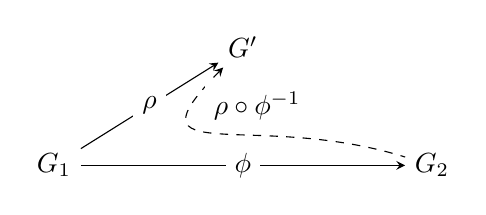
\begin{tikzpicture}[xscale=.6,yscale=.5,>=stealth]
            \node (E0) at (0, 0) {$G_1$};
            \node (E1) at (8, 0) {$G_2$};
            \draw[->] (E0) -- (E1) node[midway,fill=white] {$\phi$};
            \node (Eb) at (4, 3) {$G'$};
            \draw[->] (E0) -- (Eb) node[midway,fill=white] {$\rho$};
            \draw[<-] (Eb) edge[dashed,in=160,out=-130,looseness = 2] (E1);
            \node[fill=white] at (4.3,1.5) {$\rho \circ \phi^{-1}$};
        \end{tikzpicture}
        \caption[Zero-Knowledge protocol for graph isomorphism]{%
          The classic zero-knowledge proof of knowledge of a graph isomorphism.
        }
        \label{fig:idscheme}
    \end{center}
\end{figure}

It is relatively straightforward to check that this protocol satisfies the completeness, special soundness, and perfect honest-verifier zero-knowledge properties.


\subsection{Non-interactive ZK and signatures}

Sigma protocols are interactive protocols between a prover and a verifier, and an important feature of them is that the challenge is chosen by the verifier after the commitment has been sent. In many applications it is inconvenient to work with interactive protocols and so we want non-interactive versions of these.
One important application of non-interactive sigma protocols for hard relations is the construction of digital signatures that are existentially unforgeable under adaptive chosen-message attacks.

The best-known approach to making sigma protocol non-interactive is the Fiat-Shamir heuristic.
The basic idea of the Fiat-Shamir transform is to use a cryptographic hash function $H$ to compute the challenge, as $\chall  = H(\com)$. This can only be secure when the challenge is a bit string of sufficient length such that the soundness error is negligible. In this case, the protocol should still be sound, as the prover cannot choose $\chall$ in advance and compute a commitment that hashes to that value.

In the context of digital signatures, the Fiat-Shamir transform is as follows.
The public key of the signature scheme is an instance $x$ for a hard relation, and the secret key is a witness $w$ for the relation. To sign a message $m$, the prover runs the sigma protocol, except that it replaces the challenge by the hash value $\chall = H(m,x,\com)$, where $m$ is the message to sign.
A signature then consists of the commitment and response messages. To verify a signature, one simply recomputes the hash value and runs the verification algorithm for the sigma protocol. Intuitively, this is secure because the security properties of the hash function force the challenge to be a randomly distributed value generated after the commitment, as in the normal execution of the sigma protocol.
The $n$-special soundness of the sigma protocol provides an extractor that, by re-winding a forger in the random oracle model, allows to compute a witness from the signatures output by the forger.
The zero-knowledge property of the sigma protocol provides a simulator that allows to generate signatures in the random oracle model on messages queried by the forger to the signing oracle. Hence we have security against chosen message attacks.


In the context of post-quantum cryptography, the random oracle model must be replaced by the {quantum} random oracle model. 
%
Fiat-Shamir signatures have also been proven secure in this model under certain conditions~\cite{KLS18}, and otherwise the Unruh transform offers an alternative, albeit less efficient construction~\cite{Unruh15}. 
%\develop{Check, add reference, comment on FS security for the signature schemes discussed here}

While the Fiat-Shamir heuristic allows to construct a signature from any sigma protocol for a hard relation, not every Fiat-Shamir-style signature corresponds to a special-sound sHVZK sigma protocol.
There are two reasons for this.
First, the computational assumption(s) required for the hardness of forgery are not necessarily the same as the computational assumption of extracting a witness for a statement $x$.
Second, in the case where the signature scheme requires a computational assumption for zero-knowledge, there is a subtle difference between the definition of computational zero-knowledge for sigma protocols and the requirements for the simulator to generate signatures in the random oracle model to answer signing queries. 
Precisely, computational ZK requires computational indistinguishability for every fixed $x$, whereas for signatures the probability space in the security definition includes the random generation of $x$.

%it suffices to have a signing oracle in the average-case (e.g., that is correct for ``most'' $x$).






\section{The CSIDH setting\label{sec:CSIDH-setting}}



In this section, we discuss two sigma protocols for the natural relation coming from group actions in the specific case of CSIDH~\cite{CSIDH} (see Definition~\ref{defn:R-CSIDH} below).

%Fix a prime $p$ of the form $p = 4\ell_1 \cdots \ell_r -1$, for some integer $r$, where the $\ell_i$ are distinct small odd primes, and we let $E_0/\Field_p$ be the supersingular curve defined by $y^2 = x^3 +x $. Then the $\Field_p$-endomorphism ring of $E_0$ (and that of any curve $\Field_p$-isogenous to $E_0$) is isomorphic to $\mathbb{Z}[\sqrt{-p}]$. (Alternatively, one could work with curves whose $\Field_p$-endomorphism ring is $\mathbb{Z}[(1+\sqrt{-p})/2]$, see \cite{CD20}.) We assume that the class group $\cl(\mathbb{Z}[\sqrt{-p})]$ is generated by the ideal classes of the $r$ ideals of the form $\fl_i = (\ell_i, \sqrt{-p} - 1)$ for $i$ from $1$ to $r$. The class group $\cl(\mathbb{Z}[\sqrt{-p})]$ acts freely and transitively on the set $\Ell$ of $\Field_p$-isomorphism classes of elliptic curves with $\Field_p$-endomorphism ring $\mathbb{Z}[\sqrt{-p}]$, and that we can efficiently compute the action of the ideals classes $\overline{\fl}_1,\cdots,\overline{\fl}_r,$ and their inverses. For a vector $\bx \in \mathbb{Z}^r$ and $E \in \Ell$ we define \[ [\bx]E := \left( \prod_{i=1}^r \overline{\fl}_i^{x_i} \right) \star E  \, , \] where $\star$ is the action of the ideal class group, also known in this setting as the CSIDH action. 

Recall that the action of a vector $\bx \in \mathbb{Z}^r$ on $E \in \Ell$ is defined by \[ [\bx]E := \left( \prod_{i=1}^r {\overline{\fl}_i}^{x_i} \right) \star E  \, , \] where $\star$ is the action of the ideal class group. Note that $\star$ is computed using a sequence of isogenies of degree $\ell_i$ corresponding to the prime ideals $\fl_i$.



\begin{definition} \label{defn:R-CSIDH}
The CSIDH relation is
\[
\R[CSIDH] = \left\{ (E,\bx) \in \Ell \times \mathbb{Z}^r \,\, | \,\, [\bx]E_0 = E \right\}.
\]
\end{definition}


%\WB{reviewer says: I personally would argue adding R CSIDH to the intro is worth it but I admit it's not easy given the definition}
%\SG{I have attempted to give a brief formulation in the intro, so that at least the experts can see what it is easily.}\CP{made another suggestion}

%{\bf GAIP.} The group action inverse problem (GAIP) asks, given $E = [\bx]E_0$ to compute $\bx' \in \mathbb{Z}^r$ (possibly different from $\bx$) such that $[\bx']E_0 = E$. We assume that this problem is hard on average, when $E$ is chosen uniformly at random in $\Ell$, or when it is chosen of the form $[\bx] E_0$, for $\bx$ chosen uniformly at random from a large enough box $\{-B,\dots,B\}^r$ (large enough means $(2B+1)^r \approx \sqrt{p}$). As discussed in \cref{sec:sigma}, if GAIP is indeed hard on average for one of these distributions, then a sigma protocol for $\Rela$ can be turned into a secure signature scheme.

We now describe two sigma protocols for the relation \R[CSIDH]. The first protocol is simpler and more efficient, but it requires knowledge of the structure of the class group $\cl(\mathbb{Z}[\sqrt{-p}])$ and the relations between the ideal classes $\overline{\fl}_i$. This is a big disadvantage because (pre)computing this information is expensive, which means the first protocol can only be used for small parameters, e.g., when the order of the class group is $\approx 2^{256}$, see~\cite{CSI-FiSh}.\footnote{The structure of a class group can be computed in quantum polynomial time, so this protocol could be used with large class groups if anyone with access to a quantum computer is willing to compute a class group and publish the result (which can be verified efficiently with classical algorithms).} The second protocol is less efficient, but it does not require knowledge of the class group, and can thus be used for larger class group actions.  

\subsection{CSI-FiSh sigma protocol}

We will call the first protocol the CSI-FiSh protocol, even though a variant was already known well before the CSI-FiSh paper. It is a straightforward generalization of the graph isomorphism protocol from \cref{sec:GMW} and was already described in the group actions setting by Couveignes~\cite{Couv06},  Rostovstev and Stolbunov~\cite{RosSto}, and in more detail by De Feo and Galbraith in the CSIDH setting~\cite{SeaSign}. An optimization of the protocol that uses quadratic twists was added to the protocol in the CSI-FiSh paper~\cite{CSI-FiSh}.


In this section, we assume\footnote{All the results generalize to the more general case where the class group is not necessarily cyclic.} for simplicity that the class group $\cl(\mathbb{Z}[\sqrt{-p}])$ is cyclic with a generator $\overline{\fg}$ of known order $N$,  and that we know the discrete logarithms $a_1,\dots,a_k$ of the ideal classes $\overline{\fl}_1,\dots,\overline{\fl}_r$ with respect to $\overline{\fg}$. This includes the case of the CSIDH-512 parameter set, proposed by~\cite{CSIDH}, with $r = 74$, and where the first 73 small primes $\ell_1,\dots,\ell_{73}$ are the first 73 odd primes, and where $\ell_{74} = 587$. For this choice of prime $p$, the class group was computed by Beullens, Kleinjung, and Vercauteren~\cite{CSI-FiSh}. It turned out that the class group is cyclic of order \[N = {\scriptstyle 254652442229484275177030186010639202161620514305486423592570860975597611726191 } \, ,\] and that the ideal class of the first ideal $\fl_1 = (3,\sqrt{-p}-1) $ generates the entire class group. The discrete logarithms of the remaining $\overline{\fl}_i$ with $i > 1$, as well as a reduced basis for the relation lattice  \href{https://github.com/KULeuven-COSIC/CSI-FiSh/tree/master/classgroup_data}{are publicly available}.

Given an integer $x \in \mathbb{Z}/ N \mathbb{Z}$ and a curve $E \in \Ell$ we want to compute the action of $\overline{\fg^x}$ on $E$. Naively computing the action of $\overline{\fg}$ a total of $x$ times would require an exponential amount of time, so this is not efficient. Instead, since we know the discrete logarithms $a_i$ such that $\overline{\fg^{a_i}} = \overline{\fl}_i$ for all $i$ from 1 to $r$, we can use lattice algorithms to find a short vector $\bx \in \mathbb{Z}^r$ such that $\sum_{i=1}^r a_i x_i = x \mod N$. Once we have such a vector we can evaluate $[\bx]E$ efficiently. Asymptotically, this could be inefficient, because the lattice algorithms are too slow or produce vectors that are too large, but in practice (at least for the CSIDH-512 parameter set) this is not a problem: for CSIDH-512 the lattice algorithms are much faster than the isogeny computations, and the resulting vector $\bx$ is close to optimal. In total, computing the action of $\overline{\fg^x}$ on $E \in \Ell$ for a random $x \in \mathbb{Z}/ N \mathbb{Z}$ is only 15\% slower than computing $[\bx]E$ for a random $\bx \in [-5,5]^{74}$ (which is done in the CSIDH-512 key exchange protocol). For more details, we refer to~\cite{CSI-FiSh}.

With these details out of the way, we have a group action of $\mathbb{Z}/ N \mathbb{Z}$ on $\Ell$ (instead of a group action of $\mathbb{Z}^r$). With a mild abuse of notation, we denote the action of $x \in \mathbb{Z}/ N \mathbb{Z}$ on $E \in \Ell$ also by $[x]E$. \Cref{fig:csi-FiSh} shows the CSI-FiSh sigma protocol, which is an adaptation of the sigma protocol for graph isomorphism to this group action (replacing the action of $S_n$ on graphs of order $n$ by the action of $\mathbb{Z}/ N \mathbb{Z}$ on $\Ell$). However, a difference is that we can make the challenge space slightly larger ($\{-1,0,1\}$ instead of $\{0,1\}$), by exploiting the fact that if $E^t$ is the quadratic twist of $E = [x]E_0$, then $E^t$ is $\Field_p$-isomorphic to $[-x]E_0$. A cheating prover who does not know $x$ can win each round with probability $1/3$. The proofs that this sigma protocol is complete, 2-special sound for the relation $\R[CSIDH]$,  and honest-verifier zero-knowledge are 
straightforward; 
we refer to~\cite{CSI-FiSh}.

\begin{figure}
    \centering
    \begin{adjustbox}{minipage=0.95\linewidth,fbox,center}
    \begin{tabularx}{\textwidth}{bsB}
    \multicolumn{1}{c}{{\bf Prover}(($E,x$))} &  & \multicolumn{1}{c}{{\bf Verifier}($E$)} \\
    \\
    \quad $b \gets \mathbb{Z}/ N \mathbb{Z}$ \\
    \quad $E' \gets [b]E_0$ & & \\
     &  \multicolumn{1}{c}{ $\xrightarrow{\quad E' \quad } $ }  & \\
     & & \quad $c \gets \{-1,0,1\}$ \\
     & \multicolumn{1}{c}{ $\xleftarrow{\quad c \quad } $ } & \\ 
    \quad $r \gets b - cx \mod{N}$ & & \\
    & \multicolumn{1}{c}{ $\xrightarrow{\quad r \quad }$} & \\
    & & \quad {\bf If $c = -1$:} \\
    & & \quad \quad {\bf return} $E' = [r]E^t$ \\
    & & \quad {\bf If $c = 0$:} \\ 
    & & \quad \quad {\bf return} $E' = [r]E_0$  \\
    & & \quad {\bf If $c = 1$:} \\
    & & \quad \quad {\bf return} $E' = [r]E$ 
    \end{tabularx}
    \end{adjustbox}
    \caption{The CSI-FiSh sigma protocol. Here, and in subsequent figures, the equal sign denotes the equality predicate and the return statements return either true or false.}
    \label{fig:csi-FiSh}
\end{figure}


\subsection{CSI-FiSh non-interactive proofs/signatures}

We can obtain a non-interactive proof for the CSIDH relation by applying the Fiat-Shamir transform to the sigma protocol of \cref{fig:csi-FiSh}, after amplifying the soundness. The resulting protocol is called CSI-FiSh (Commutative Supersingular Isogeny Fiat-Shamir). Since the base sigma protocol has a challenge space of size 3, we need to repeat the protocol $k = \lceil \lambda/\log3 \rceil$ times to get $\lambda$ bits of security. Note that the verifier can compute the $E'$ himself, so they do not need to be included in the proof. Therefore, a proof is of the form $\sigma = \{ c^{(i)},r^{(i)} \}_{i \in [k]}$. For $\lambda$ bits of classical security, we need $N \approx 2^{2\lambda}$, so the total proof size is \[
k ( 2 + 2\lambda ) \approx 1.26 \lambda^2 \text{ bits} \, .
\]

We can use this non-interactive proof as a signature scheme. However, if the goal is to obtain efficient signatures, it is possible to significantly reduce the signature size at the cost of increasing the size of the public keys.

{\bf Protocol with larger challenge space.} \label{sec:multiple_keys} In a nutshell, the idea is that instead of letting the public key be a single curve $E$, we let the public key consist of $S$ curves $E_1 = [x_1]E_0, \dots, E_S = [x_S]E_0$, where the $x_1, \dots, x_S$ are the new secret key. The new sigma protocol is similar to that of \cref{fig:csi-FiSh}, but has a challenge space $\{-S,\dots,S\}$ (of size $2S+1$), and in response to challenge $c$, the prover sends a response $r$, such that $[r]E_c = E'$ if ($c \ge 0$), or such that $[r]E_{-c}^t = E'$ in case $c \leq 0$. 
One can show in the random oracle model that a forger against this protocol can be turned into an algorithm that takes as input the curves $E_1, \dots, E_S$ and outputs a triple $(i,j,x)$ such that $1 \le i < j \le S$ and $[x]E_i = E_j$; this is believed to be a hard problem but it is not the problem of computing a witness for the relation $\R[CSIDH]$ so the protocol is not a proof of knowledge for this relation.
The advantage of this sigma protocol is that the challenge space is larger, so the protocol only needs to be repeated $\lambda/\log(2S+1)$ times for soundness error $2^{-\lambda}$. The signature size of the new signature is approximately \[
\frac{2}{\log(2S+1)} \lambda^2 \text{ bits} \,.
\]
However, the size of the public key is now $4S \lambda$. So the parameter $S$ gives a trade-off between small signatures (large $S$) and small public keys (small $S$). For more details (and a technique based on Merkle trees to reduce the size of the public key) we refer to the SeaSign or CSI-FiSh papers~\cite{SeaSign,CSI-FiSh}.


\iffalse
{
\color{gray}
{\bf Protocol with larger challenge space.} \label{sec:multiple_keys}
[WARD: I think we discussed that we would not talk about this, so I'll summarize this in one or two sentences.] 

In a nutshell, the idea is that instead of letting the public key be a single curve $E$, we let the public key consist of $S$ curves $E_1 = [x_1]E_0, \dots, E_S = [x_S]E_0$. The new sigma protocol is similar to that of \cref{fig:csi-FiSh}, but has a challenge space $\{-S,\dots,S\}$ (of size $2S+1$), and in response to challenge $c$, the prover sends a response $r$, such that $[r]E_c = E'$ if ($c \ge 0$), or such that $[r]E_{-c}^t = E'$ in case $c \leq 0$. One can check that this is a correct and honest-verifier zero-knowledge sigma protocol for the relation \[
\Rela^S  = \left \{ ((E_1,\dots,E_S),(x_1,\dots,x_S)) \,\, \middle | \,\, [x_i]E_0 = E_i \quad  \forall i \in \{1,\dots,S\} \right \} \,.
\]
Moreover, this protocol has relaxed special soundness   for the relaxed relation \[
{\Rela'}^S = \left \{ ((E_1,\dots,E_S),(x_1,i,j)) \,\, \middle | \,\, ([x]E_i = E_j \vee [x]E_i = E^t_j) \quad \wedge \quad i \ne j \right \} \,,
\] because given two accepting transcripts of the protocol, one can recover $x$ such that $[x]E_i = E_j$ or $[x]E_i = E^t_j$ for some $i \neq j \in \{0, \dots, S\}$. One can prove that breaking the relaxed relation is equally hard as breaking the group action inverse problem (GAIP). This means that applying the Fiat-Shamir protocol to the new sigma protocol results in a secure signature scheme. (Because if someone could forge signatures, they could solve GAIP, which is assumed to be difficult). 

The advantage of this sigma protocol is that the challenge space is larger, so the protocol only needs to be repeated $\lambda/\log(2S+1)$ times. The signature size of the new signature is approximately \[
\frac{2}{\log(2S+1)} \lambda^2 \text{ bits} \,.
\]

However, the size of the public key is now $4S \lambda$. So the parameter $S$ gives a trade-off between small signatures (large $S$) and small public keys (small $S$). For more details (and a technique based on Merkle trees to reduce the size of the public key) we refer to the SeaSign or CSI-FiSh papers~\cite{SeaSign,CSI-FiSh}.

}
\fi

\subsection{SeaSign sigma protocol}

If the structure of the class group of $\mathbb{Z}[\sqrt{-p}]$ is not known, then we cannot efficiently compute the action of $\mathbb{Z}/N \mathbb{Z}$ on $\Ell$, so we cannot directly use the CSI-FiSh protocol. The naive way to solve this problem would be to just work with the action of $\mathbb{Z}^r$ instead: To prove knowledge of $\bx$ such that $E = [\bx]E_0$, the prover picks $\bb \in [-B,B]^r$ uniformly at random and sends $[\bb]E_0$ to the verifier, who responds with a challenge $c \in \{-1,0,1\}$, and then the prover sends his response $\br = \bb - c\bx$. Unfortunately, this sigma protocol is not zero knowledge, because in the case $c = 1$, the response is biased towards $-\bx$, and if $c = -1$, the response is biased towards $\bx$. After observing a number of executions of the protocol, an attacker could just compute the average of $- c \br$ to get a good estimate of $\bx$.

In the CSI-FiSh case we chose $b$ uniformly at random, so the response $r = b + cx \mod N$ does not reveal information about $x$. In the new protocol, since $\mathbb{Z}^r$ is infinite, we cannot choose $\bb$ uniformly at random, so the response $\br = \bb + c \bx$ leaks information about $\bx$.



One approach to  the problem is to sample $\bb$ from a box $[-\delta B,\delta B]^r$ where $\delta > 1$, which is larger than the box $[-B,B]^r$ from which the secret $\bx$ is sampled. The hope is that if $\delta B$ is much larger than $B$, then the distribution of $\bb + \bx$ is close to the distribution of $\bb$, so it does not leak information about $\bx$. Unfortunately, to make the two distributions indistinguishable $\delta B$ would need to be exponentially larger than $B$. This is impractical because then evaluating the action of $[\bb]E_0$ would take an exponential amount of time.

However the following observation can help us: The response $\br = \bb - c \bx$ can take values in $[-(\delta + 1)B,(\delta + 1)B]$, but $\br$ only leaks information about $\bx$ if $\br$ is close to the boundary of this box. For example, if in the $c = 1$ case one of the coefficients $r_i$ is equal to $-(\delta+1)B$, then this reveals that $x_i = -B$. Conversely, if $\br$ is sufficiently far away from the boundary, then it does not leak information: If $\br \in [-(\delta-1) B, (\delta-1) B]^r$ (which happens with probability $\left( \frac{2(\delta-1) B+1}{2\delta B+1} \right)^r \approx \left(1 - \frac{1}{\delta}\right)^r$), then all values of $\bx$ are consistent with $\br$, and the probability of seeing the response $\br$ is independent of $\bx$, so $\br$ does not reveal any information about $\bx$. 

Using this observation, we can design a sigma protocol with aborts (a concept introduced by Lyubashevsky~\cite{FSWithAborts}) as follows: we pick $\delta$ large enough such that with reasonably large probability (e.g. at least $1/2$), the response $\br$ lies in the ``safe'' box $[-(\delta-1) B, (\delta-1) B]^r$. Before the prover sends a response $\br$ they first check if $\br$ lies in $[-(\delta-1) B, (\delta-1) B]^r$. If this is the case, then the prover sends the response to the verifier, and otherwise, the prover aborts the sigma protocol to avoid leaking information. This way, we guarantee that the responses do not leak any information about $\bx$. 

The protocol is summarized in \cref{fig:SeaSign}. We can prove that the protocol aborts with probability $\epsilon$ close to $1-\left(1-\frac{1}{\delta} \right)^r$, that the protocol is correct (i.e. if in an honest execution the prover does not abort, then the verifier will accept), that the protocol has special soundness, and that the protocol has non-abort honest verifier zero-knowledge, meaning that non-aborting transcripts of the protocol can be simulated without knowledge of $\bx$.

\begin{figure}
    \centering
    \begin{adjustbox}{minipage=\linewidth,fbox,center}

    \begin{tabularx}{\textwidth}{Bsb}
    \multicolumn{1}{c}{{\bf Prover}(($E,\bx$))} &  & \multicolumn{1}{c}{{\bf Verifier}($E$)} \\
    \\
    \quad $\bb \gets [-\delta B, \delta B]^r $ \\
    \quad $E' \gets [\bb]E_0$ & & \\
     &  \multicolumn{1}{c}{ $\xrightarrow{\quad E' \quad } $ }  & \\
     & & \quad $c \gets \{-1,0,1\}$ \\
     & \multicolumn{1}{c}{ $\xleftarrow{\quad c \quad } $ } & \\ 
    \quad $\br \gets \bb - c\bx$ & & \\
    \quad {\bf If $\br \not \in [-(\delta-1)B,(\delta-1)B]^r$:} && \\
    \quad \quad Prover aborts & & \\
    & \multicolumn{1}{c}{ $\xrightarrow{\quad \br \quad }$} & \\
    & & \quad {\bf If $c = -1$:} \\
    & & \quad \quad {\bf return} $E' = [\br]E^t$ \\
    & & \quad {\bf If $c = 0$:} \\ 
    & & \quad \quad {\bf return} $E' = [\br]E_0$  \\
    & & \quad {\bf If $c = 1$:} \\
    & & \quad \quad {\bf return} $E' = [\br]E$ 
    \end{tabularx}
    \end{adjustbox}
    \caption{The SeaSign sigma protocol with abort.}
    \label{fig:SeaSign}
\end{figure}


\subsection{SeaSign non-interactive proofs/signatures.}

Just like with a normal sigma protocol, the soundness of a sigma protocol with abort can be amplified by repeating the protocol $k = \lceil \lambda / \log 3 \rceil$ times in parallel. However, this increases the probability of an abort from $\epsilon$ to $1-(1-\epsilon)^k$. We can choose $\delta = kr$, such that the probability that none of the $k$ repetitions of the sigma protocols abort is approximately $(1-\frac{1}{\delta})^{kr} \approx 1/e$.

Then, we can transform the amplified sigma protocol into a signature scheme with the Fiat-Shamir transform. If during the generation of a signature the prover aborts, then the signer can just restart the signing algorithm. As long as the success probability is not too small (e.g., $\approx 1/e$ if $\delta = kr$) the signing algorithm will succeed after a reasonable number of attempts.

{\bf Optimizing SeaSign.} The technique of using multiple curves in the public key, which we described in \cref{sec:multiple_keys} can also be used to reduce the signature size of SeaSign (at the cost of larger keys). In fact, this technique was introduced in the SeaSign paper.

Note that if $c=0$, then the response is just $\br = \bb$, which does not leak information about $\bx$. Therefore, the prover does not need to abort if $\br$ lies outside of the ``safe'' box $[-(\delta-1)B,(\delta-1)B]^r$. This optimization reduces the rate of aborts, which means we can reduce $\delta$, which in turn makes the signing algorithms faster (and the signatures slightly smaller). This optimization was described in a paper by Decru, Panny, and Vercauteren~\cite{FasterSeaSign}, along with some additional optimizations which are beyond the scope of this survey.



\section{The generic supersingular setting \label{sec:SIDH-setting}}



We now move to settings that are specific to supersingular curves.
We focus on the relations $\R[isog]$ and $\R[deg]$.
%, and later we briefly discuss the challenges of $\R[SIDH]$.
As mentioned in Section~\ref{sec:isog-graph} it suffices to consider elliptic curves defined over a finite field $\F_{p^2}$.
%, as we saw that any supersingular curve is isomorphic to one defined over a quadratic finite field.
Lacking a well behaved group action on the set of supersingular curves, we have to get more creative in order to define secure protocols.

Along with the SIDH key exchange, De Feo, Jao and Pl\^{u}t~\cite{DFJP14} sketched the first sigma protocol to prove knowledge of an isogeny between two supersingular curves over $\F_{p^2}$, provided $p$ is an ``SIDH prime''.
We start by presenting this simple protocol, which we refer to as DFJP.
We highlight some issues with its soundness and zero-knowledge, and explain how to fix them, following De Feo, Dobson, Galbraith and Zobernig~\cite{DFDGZ21}.
Then, we present a recent generalization of DFJP which applies to any characteristic and achieves statistical zero-knowledge~\cite{cryptoeprint:2022/1469}.
Finally, we discuss some open questions.


\subsection{The DFJP protocol}\label{sec:DFJP}

We are in the SIDH setting, hence $p = 2^n 3^m f - 1$ and supersingular curves over $\F_{p^2}$ have group structure isomorphic to $(\Z/(p+1)\Z)^2$.
We can thus efficiently construct SIDH squares
%
\begin{equation}
    \label{eq:sidh-pok}
    \tikz[x=2cm,y=-1.5cm,baseline=-.75cm]{
    \node (E0) at (0,0) {$E_0$};
    \node (E1) at (1,0) {$E_1$};
    \node (E2) at (0,1) {$E_2$};
    \node (E3) at (1,1) {$E_3$};
    \draw[->] (E0) edge node[above] {$\phi$} (E1)
    (E0) edge node[left] {$\psi$} (E2)
    (E1) edge node[right] {$\psi'$} (E3)
    (E2) edge node[above] {$\phi'$} (E3);
    }
\end{equation}
%
where the degrees of $\phi$ and $\psi$ are coprime (usually degrees $2^n$ and $3^m$ respectively).

Suppose a prover wants to prove knowledge of an isogeny $\phi : E_0 \to E_1$ of degree $d = 2^n$.
The idea of DFJP is simply to choose a random $\psi$ of degree co-prime to the degree of $\phi$, commit to $(E_2,E_3)$, and then reveal some, but not all, of $\psi,\psi',\phi'$.
They observe that revealing $(\psi,\phi')$ or $(\psi',\phi')$ is insecure, as that would immediately reveal the secret $\phi$ by pushing $\phi'$ (or its dual) through $\psi$ (or $\psi'$).
However they note that revealing $\phi'$ or $(\psi,\psi')$ only appears to leak a limited amount of information on $\phi$, and thus suggest the following protocol:
\begin{enumerate}
    \item The prover chooses a random cyclic group $G = \ker(\psi)$ of order $D=3^m$, sets $E_2=E_0/G$ and $E_3 = E_1/\phi(G)$ and so constructs the commutative diagram~\eqref{eq:sidh-pok}, and sends $(E_2,E_3)$ to the verifier;
    \item The verifier challenges with a random bit $\chall\in\{0,1\}$;
    \item The prover responds with $(\ker(\psi),\ker(\psi'))$ if $\chall=0$, and with $\ker(\phi')$ otherwise;
    \item If $\chall=0$ the verifier checks that $E_2 \cong E_0/\ker(\psi)$ and $E_3 \cong E_1/\ker(\psi')$, otherwise it checks that $E_3 \cong E_2/\ker(\phi')$.
\end{enumerate}

There are two issues with the above idea.
First, having binary challenges, it must be repeated $\lambda$ times to achieve a soundness error of $2^{-\lambda}$, and is thus not particularly efficient.
Second, as we explain next, it is not zero-knowledge, at least not for the \R[deg] relation.

\begin{remark}
    DFJP represent $\phi$ (resp.\ $\psi$) by a generator $K_\phi$ (resp.\ $K_\psi$) of its kernel, and then represent $\phi'$ (resp.\ $\psi'$) by $\psi(K_\phi)$ (resp.\ $\phi(K_\psi)$). This representation conveys more information than necessary, and makes the protocol provably less secure. We instead assume isogenies are represented by their whole kernel, which in practice is done by transmitting a kernel generator chosen at random, or deterministically in a way that only depends on the isogeny.
\end{remark}

\subsubsection{Zero Knowledge.} 
The reason the DFJP protocol is not zero-knowledge is that the pair $(\ker(\psi), \phi(\ker(\psi)))$ revealed when $\chall = 0$ leaks enough information to recover the witness $\phi$.
Indeed, thanks to~\cite[Lemma~1]{10.1007/978-3-030-95312-6_14}, three such pairs are sufficient to compute a torsion basis $\langle P,Q\rangle = E_0[D]$ and points $P' = \lambda\phi(P)$, $Q' = \lambda\phi(Q)$ for some $\lambda$ such that $\lambda^2 = 1 \bmod D$.
But $\lambda = \pm 1$ because $D = 3^m$, hence the attacks of Castryck and Decru~\cite{CD22}, Maino and Martindale~\cite{MM22}, and Robert~\cite{Rob22} apply and recover $\phi$.

Note that $D = 3^m$ is important here.
If, instead, $D$ is taken to contain many distinct prime factors, like in~\cite{cryptoeprint:2023/013}, there are exponentially many possibilities for $\lambda$, and it is not currently known how to systematically apply the SIDH attacks to this case.
Indeed, (roughly) following De Feo, Jao and Plût, we can prove that their protocol is zero-knowledge for the \R[M-SIDH] relation, and is thus a non-trivial proof of knowledge for instances where \R[M-SIDH] is still believed to be hard.

There is also a second, less dramatic issue associated to the $\chall = 1$ case.
Indeed, the response $\ker(\phi') = \psi(\ker(\phi))$ appears to be correlated to $\phi$, and thus hard to simulate without knowledge of the witness.
DFJP simulate $\ker(\phi')$ with a randomly chosen group, thus reducing zero-knowledge to the hardness of the following computational problem, stating that it is difficult to distinguish pairs of ``parallel'' isogenies from random pairs of isogenies of the same degree.

\begin{definition}[Decisional Supersingular Product Problem (DSSP)]\label{defn:DSSP}
    Let $E_0$ and $E_1$ be supersingular curves over $\F_{p^2}$ and let $\phi :E_0 \to E_1$ be an isogeny of degree $d$.
    Let $D$ be an integer coprime to $d$.
    The DSSP problem is, knowing $\phi$, to distinguish between the two following distributions:
    \begin{itemize}
        \item $D_0 = \{ \phi' : E_2 \to E_3 \}$, where $\psi : E_0 \to E_2$ is uniformly sampled among all cyclic $D$-isogenies starting from $E_0$, and $\ker(\phi') = \psi(\ker(\phi))$; and
        \item $D_1 = \{ \phi' : E_2 \to E_3 \}$, where $\psi : E_0 \to E_2$ is sampled as above, and $\phi'$ is a uniformly sampled cyclic $d$-isogeny starting from $E_2$.
    \end{itemize}
\end{definition}


\subsubsection{Soundness.}
DFJP claim their protocol is sound for the weaker relation $\R[deg]$.
Unfortunately, this claim was independently shown to be wrong by De Feo, Dobson, Galbraith and Zobernig~\cite{DFDGZ21} and by Ghantous, Pintore and Veroni~\cite{GPV21}, with explicit counterexamples presented in both papers.

It is possible, and in fact very simple, to show that DFJP is 2-special sound for $\R[isog]$, i.e.\ that it is a proof of knowledge of \emph{an isogeny}, without any further qualifications. 


\begin{lemma}
    The DFJP protocol is a 2-special-sound proof of knowledge for the relation
    $\R[isog]  = \bigl\{ \bigl((E_0, E_1),\phi \bigr) \,\big\vert\, \phi : E_0 \to E_1 \text{ is an arbitrary isogeny}\bigr\}$.
\end{lemma}
\begin{proof}
Consider an extractor that is given responses to two challenges for the same commitment $(E_2,E_3)$.
The extractor has isogenies  $\psi : E_0 \to E_2$,  $\psi' : E_1 \to E_3$ and the isogeny $\phi':E_2 \to E_3$.
Then the isogeny $\widehat{\psi'} \circ \phi' \circ \psi $ is an isogeny from $ E_0 $ to $E_1$.
\end{proof}

Additionally, Ghantous, Pintore, and Veroni~\cite{GPV21} prove that, in some circumstances, DFJP is sound for $\R[deg]$ according to a weaker definition of 2-special soundness that assumes the existence of a witness.
In summary DFJP is a sound protocol for \R[isog], and is computationally ZK for \R[M-SIDH], which may or may not be a hard relation.
While this may be enough for some applications, e.g., signatures, it falls short in many ways.


\subsection{A sigma protocol for $\R[deg]$}\label{sec:R-deg}

De Feo, Dobson, Galbraith and Zobernig~\cite{DFDGZ21} modified the DFJP protocol to achieve both soundness and ZK for the relation $\R[deg]$.

The first fix concerns ZK: to avoid leaking the action of $\phi$ on $E_0[D]$, they move from binary to ternary challenges, revealing only one of $\psi$, $\psi'$ or $\phi'$ at a time.
The idea of ternary challenges for isogeny problems originates in the work of Boneh, Kogan and Woo~\cite{BKW20}.
This is not sufficient: the commitment $(E_2,E_3)$ still leaks information.
To prevent this leakage they resort to a statistically hiding commitment scheme \Com, to securely hide the values of $E_2$ and $E_3$ until the response step.\footnote{Such a commitment scheme can be easily instantiated as $\Com(m;r) = H(m \Vert r)$, where $H$ is a hash function and $r$ is a sufficiently long random string.}

The second fix concerns soundness, and is more involved.
The main obstacle to extracting $\phi$ in DFJP is that the three sides $\psi,\psi',\phi'$ of a diagram do not necessarily imply the existence of a fourth side of degree $d$:
%
\begin{equation*}
    \tikz[x=2cm,y=-1.5cm]{
    \node (E0) at (-0.5,0) {$E_0$};
    \node (E1) at (1.5,0) {$E_1$};
    \node (E2) at (0,1) {$E_2$};
    \node (E3) at (1,1) {$E_3$};
    \draw[->] (E0) edge[dotted] node[above] {??} (E1)
    (E0) edge node[left] {$\psi$} (E2)
    (E1) edge node[right] {$\psi'$} (E3)
    (E2) edge node[above] {$\phi'$} (E3);
    }
\end{equation*}
%
The existence of $\phi$ parallel to $\phi'$ is guaranteed if and only if $\widehat\psi$ and $\widehat\psi'$ are proven to be parallel with respect to $\phi'$.
The key idea then is to ``flip the SIDH square'' and to treat $\phi':E_2\to E_3$ as the base for the square.
By publishing torsion point information associated to $E_2$ and $E_3$, one can prove that $\widehat\psi$ and $\widehat\psi'$ are indeed parallel.

Putting all ideas together gives the following protocol (also see Figure~\ref{fig:R-deg-proof}):


\begin{enumerate}
    \item The prover:
    \begin{itemize}
        \item Chooses a random cyclic group $G = \ker(\psi)$ in $E_0$ of order $D$, and constructs the commutative diagram~\eqref{eq:sidh-pok} (meaning: constructs $\phi' : E_2 \to E_3$ with $\ker(\phi') = \psi( \ker( \phi ))$).
        \item Chooses a random basis $P_2,Q_2$ of $E_2[D]$, computes $P_3 = \phi'(P_2), Q_3 = \phi'(Q_2)$.
        \item Computes integers $(a,b)$ such that $\ker(\widehat\psi) = \langle [a]P_2 + [b]Q_2\rangle$.
        \item Sends commitments $\Com_L = \Com(E_2,P_2,Q_2; r_L)$, $\Com_R = \Com(E_3,P_3,Q_3; r_R)$ and $\Com = \Com(a,b; r)$ to the verifier;
    \end{itemize}
    \item The verifier challenges with a random value $\chall\in\{-1,0,1\}$;
    \item The prover opens:
    \begin{itemize}
        \item $\Com_L$ and $\Com$ if $\chall = -1$,
        \item $\Com_R$ and $\Com$ if $\chall = 0$,
        \item $\Com_L$ and $\Com_R$ if $\chall = 1$, and additionally sends $\ker(\phi')$.
        Note that in practice one usually sends a generator for $\ker(\phi')$, in which case this generator should be sampled uniformly from the set of all generators of the subgroup;
    \end{itemize}
    \item The verifier checks that the opened commitments are well formed, and:
    \begin{itemize}
        \item that $E_0 = E_2/\langle [a]P_2 + [b]Q_2\rangle$ if $\chall = -1$,
        \item that $E_1 = E_3/\langle [a]P_3 + [b]Q_3\rangle$ if $\chall = 0$,
        \item that $E_3 = E_2/\ker(\phi')$ and that $P_3 = \phi'(P_2), Q_3 = \phi'(Q_2)$ if $\chall = 1$.
    \end{itemize}
\end{enumerate}



\begin{figure}
    \centering
    \begin{adjustbox}{minipage=1.3\linewidth,fbox,center}
    \begin{tabularx}{\textwidth}{bsb}
    \multicolumn{1}{c}{{\bf Prover}(($E_0,E_1,d,D),\phi$)} &  & \multicolumn{1}{c}{{\bf Verifier}($E_0,E_1,d,D$)} \\
    \\
    Choose random cyclic group $G \subseteq E_0$ of order $D$ \\
    Define $\psi : E_0 \to E_2$ with kernel $G$ and construct the diagram~\eqref{eq:sidh-pok} \\
    Choose a random basis $P_2,Q_2$ of $E_2[D]$ \\
    Set $P_3 \gets \phi'(P_2), Q_3 \gets \phi'(Q_2)$ \\
     Compute integers $(a,b)$ such that $\ker(\widehat\psi) = \langle [a]P_2 + [b]Q_2\rangle$ \\
     Choose random $r_L$, $r_R$, $r$ \\
     Set $\Com \gets \Com(a,b; r)$, $\Com_L \gets \Com(E_2,P_2,Q_2; r_L)$, $\Com_R \gets \Com(E_3,P_3,Q_3; r_R)$   \\   
    \quad  & & \\
     &  \multicolumn{1}{c}{ $\xrightarrow{\quad \Com_L, \Com_R, \Com \quad } $ }  & \\
     & & \quad $\chall \gets \{-1,0,1\}$ \\
     & \multicolumn{1}{c}{ $\xleftarrow{\quad \chall \quad } $ } & \\ 
     {\bf If} $\chall = -1$: $\resp \gets $ opening of $\Com_L, \Com$ & & \\
     {\bf If} $\chall = 0$: $\resp \gets $ opening of $ \Com_R, \Com$ & & \\
     {\bf If} $\chall = 1$: $\resp \gets $ opening of $\Com_L, \Com_R$, and  $\ker(\phi')$ & & \\
    & \multicolumn{1}{c}{ $\xrightarrow{\quad \resp \quad }$} & \\
    & & Check that opened commitments are well \\
    & &  formed, and
    $(P_2,Q_2)$ and/or $(P_3,Q_3)$ are $D$-torsion bases, and
    $\gcd(D,a,b)=1$\\
    & &  {\bf If} $\chall = -1$: \\
    & &  \quad {\bf return} $E_0 = E_2/\langle [a]P_2 + [b]Q_2\rangle$ \\
    & &  {\bf If} $\chall = 0$: \\ 
    & &  \quad {\bf return} $E_1 =  E_3/\langle [a]P_3 + [b]Q_3\rangle  $  \\
    & &  {\bf If} $\chall = 1$: \\
    & & \quad Check that $\#\ker(\phi') = d$\\
    & & \quad Construct $\phi'$ from  $\ker(\phi')$ \\
    & &  \quad {\bf return} $E_3 =   E_2/\ker(\phi')$ \\
     & &  \quad \quad and $P_3 = \phi'(P_2)$ \\
    & &  \quad \quad and $ Q_3 = \phi'(Q_2)$ \\
    \end{tabularx}
    \end{adjustbox}
    \caption{The sigma protocol for $\R[deg]$.}
    \label{fig:R-deg-proof}
\end{figure}





\begin{proposition}
    The protocol of Figure~\ref{fig:R-deg-proof} is a computationally ZK 3-special sound proof of knowledge for the relation
    \[\R[deg] = \bigl\{ \bigl((E_0, E_1, d), \phi\bigr) \,\big\vert\, \phi : E_0 \to E_1 \text{ is an isogeny of degree } d \bigr\},\]
    assuming DSSP is hard and $\Com$ is a statistically hiding and computationally binding commitment scheme.
\end{proposition}
\begin{proof} (Sketch)
    Correctness is similar to DFJP. The only additional property to check is that, if the SIDH square is generated honestly, one can efficiently find integers $(c,d)$ such that $\ker(\widehat\psi) = \langle [a]P_2 + [b]Q_2\rangle$ and $\ker(\widehat\psi') = \langle [a]P_3 + [b]Q_3\rangle$.
    A generator for $\ker(\widehat\psi)$ can be found by pushing $E_0[D]$ through $\psi$, then the integers $(a,b)$ can be computed by solving a generalized discrete logarithm in $E_2[D]$, which is easy because $D$ is smooth.
    Then $\ker(\widehat\psi') = \langle [a]P_3 + [b]Q_3\rangle$ follows from the fact that $\psi$ and $\psi'$ are parallel, and thus $\ker(\widehat\psi') = \phi'(\ker(\widehat\psi))$.
    
    \emph{Zero Knowledge.} The simulator for the case $\chall = -1$ picks a random isogeny $\psi:E_0\to E_2$, a random basis $(P_2,Q_2)$, computes $(a,b)$, and finally computes the commitments $\Com_L$ and $\Com$ as in the protocol.
    As the commitment $\Com_R$ will not be opened, it is replaced by a random value.
    
    The case $\chall = 0$ is nearly identical, but with the goal of ensuring $\Com_R$ and $\Com$ can be opened in the protocol.
    
    Finally, the case $\chall = 1$ is simulated by taking a random $\psi:E_0\to E_2$, then a random $\phi':E_2\to E_3$ not necessarily parallel to $\phi$, a random basis $\langle P_2,Q_2\rangle = E_2[D]$, and points $P_3 = \phi'(P_2)$ and $Q_3 = \phi'(Q_2)$.
    The commitment $\Com$ will not be opened and is replaced by a random value.
    Like in DFJP, this part of the simulation is only indistinguishable from the real protocol assuming DSSP is hard.
    
    \emph{Soundness.} Because the protocol uses ternary challenges, we show it is 3-special sound.
    Since the commitment scheme $\Com$ is computationally binding, the openings of the commitments match in each of the three valid transcripts. Hence, we extract $\widehat\psi$, $\widehat\psi'$ and $\phi'$, with the additional property that $\ker(\widehat\psi') = \phi'(\ker(\widehat\psi))$.
    Hence $\widehat\psi$ and $\widehat\psi'$ are parallel, proving the existence of a $d$-isogeny $\phi$ with kernel $\widehat\psi(\ker(\phi'))$ parallel to $\phi'$. \qed
\end{proof}


Note that a cheating prover can correctly answer any two of the challenges without knowing the witness, so the soundness error for this protocol is $2/3$.



\paragraph{Sigma protocols for \R[SIDH] and \R[M-SIDH].}
In the same work~\cite{DFDGZ21}, De Feo, Dobson, Galbraith and Zobernig further modify the previous protocol to achieve a ZK proof of knowledge for the relation \R[SIDH], i.e.\ the knowledge of an SIDH secret key.
The idea is, roughly, to run two correlated instances of the protocol, and to let the verifier check that they are both consistent with the torsion point information that is part of the public key.
While this protocol is not anymore relevant for SIDH/SIKE, a simple tweak yields a proof of knowledge for \R[M-SIDH] (see Basso~\cite{Bas23}), which is non-trivial in cases where \R[M-SIDH] is thought to be hard.

%This protocol can be used, for example, to counter the GPST adaptive attack, thus yielding a secure non-interactive key exchange based on SIDH.
%
%As DFJP is already ZK with respect to $\R[SIDH]$, it would be tempting to start from it and add more data to boost soundness.
%Unfortunately, it seems to be hard to boost soundness of DFJP without degrading ZK, thus~\cite{DFDGZ21} proceeds differently, by starting from the protocol for $\R[deg]$ in Figure~\ref{fig:R-deg-proof} which has ternary challenges.
%Hence the resulting protocol also has ternary, rather than binary, challenges.
%
%Recall that the goal is to prove knowledge of an isogeny $\phi : E_0 \to E_1$ such that $\phi(P_0) = P_1$ and $\phi(Q_0) = Q_1$, where $(P_0,Q_0)$ is a basis of $E_0[D]$, and thus $(P_1,Q_1)$ is a basis of $E_1[D]$.
%The protocol for $\R[deg]$ given above proves the existence of $\phi : E_0 \to E_1$, but nothing more.
%Our goal is to add enough information to the protocol to prove that $P_1,Q_1$ are the correct images of $P_0,Q_0$ under the extracted witness $\phi$.
%We do this through several refinements.
%
%\paragraph{Going around the square.}
%The first step is to convince the verifier that some point $R_0\in E_0[D]$ is mapped by $\phi$ to some point $R_1\in E_1[D]$.
%Because the verifier never sees $\phi$, we need to find a way that exploits $\psi$, $\psi'$ and $\phi'$.
%
%Let $R_0$ be a generator of $\ker(\psi)$, then there exists a point $R_2 = [c']P_2 + [d']Q_2$ such that $\widehat\psi(R_2) = R_0$ (here $P_2,Q_2$ are as in Figure~\ref{fig:R-deg-proof}).
%Define $R_3 = [c']P_3 + [d']Q_3 = \phi'(R_2)$ and let $R_1 = \widehat\psi'(R_3)$.
%By definition $\phi\circ\widehat\psi = \widehat\psi'\circ\phi'$, thus, going around the square, we see that $R_1 = \phi(R_0)$.
%
%These conditions can be checked separately by the verifier in each of the three challenges, provided it is given the integers $(c',d')$ in response to $\chall=-1,0$.
%
%\paragraph{Adding torsion point information}
%Writing $R_0$ as $[a]P_0 + [b]Q_0$, it follows that $R_1 = [a]P_1 + [b]Q_1$, if $P_1,Q_1$ are the correct images of $P_0,Q_0$.
%Thus we modify the protocol by having the prover commit to $(a,b,c',d')$ and then open this commitment in the cases $\chall=-1,0$.
%The verifier will check consistency by verifying that $[a]P_0 + [b]Q_0 = \widehat\psi([c']P_2 + [d']Q_2)$ if $\chall = -1$, or that  $[a]P_1 + [b]Q_1 = \widehat\psi'([c']P_3 + [d']Q_3)$ if $\chall = 0$.
%
%By 3-special soundness, this is sufficient to prove that $\phi$ maps some linear combination of $P_0,Q_0$ to the same linear combination of $P_1,Q_1$.
%Said otherwise, $P_1,Q_1$ are the correct images, up to multiplication by a $2\times 2$ matrix with eigenvector $(a\;b)$.
%Still far from enough for $\R[SIDH]$.
%
%\paragraph{Doubling the square.}
%Informally, there is a 2-dimensional ``space'' of false bases $(P_1,Q_1)$ that a cheating verifier could try to convince the verifier of.
%The modifications above convince the verifier of the correctness of a ``line'', and thus restrict the freedom of the cheating prover to a single dimension.
%It stands to reason that repeating the protocol twice for ``linearly independent'' lines should leave no freedom to the cheating prover, and thus prove that $(P_1,Q_1)$ are indeed the images of $(P_0,Q_0)$.\footnote{One must be careful with this abuse of linear algebra terminology, because $E[D]$ is only a $(\Z/D\Z)$-module.}
%
%The next modification is thus to construct two ``linearly independent'' SIDH squares on top of $\phi: E_0 \to E_1$, and run the same sigma protocol simultaneously on both of them.
%Concretely, the prover picks random $R_{0,0} = [a_0]P_0 + [b_0]Q_0$ and $R_{0,1} = [a_1]P_0 + [b_1]Q_0$, subject to the condition that $a_0b_1-a_1b_0$ is invertible modulo $D$.
%They define $\psi_0 : E_0 \to E_0/\langle R_{0,0}\rangle$ and $\psi_1 : E_0 \to E_0/\langle R_{0,1}\rangle$, and construct the associated SIDH squares.
%They then run the same protocol described above for both squares, using the same ternary challenge $\chall$ for both.
%The verifier must additionally check that $a_0b_1-a_1b_0$ is invertible modulo $D$.
%
%\paragraph{Ensuring consistency of the two squares.}
%This is still not enough.
%Suppose there are two isogenies $\phi,\chi: E_0 \to E_1$ of the same degree.
%A cheating prover could use one for the first square and the other for the second square, potentially convincing the verifier of false information on the images of $(P_0,Q_0)$.
%It is thus necessary to add information to prove that the extracted isogeny is the same in both squares.
%
%In the protocol for $\R[deg]$ we had that the extracted isogeny $\phi$ has $\ker(\phi) = \widehat\psi(\ker(\phi'))$.
%In the doubled protocol is thus sufficient to prove that
%\[\widehat\psi_0(\ker(\phi_0')) = \widehat\psi_1(\ker(\phi_1')).\]
%This is done, again, by publishing torsion point information: the prover starts by choosing a random basis $(U,V)$ of $E_0[d]$, computing $U_i = \phi_i(U), V_i = \phi_i(V)$ for $i\in\{0,1\}$ and committing to $(U_0,V_0,U_1,V_1)$.
%When it answers $\chall = 1$, it computes integers $(e,f)$ such that $\ker(\phi) = \langle [e]U + [f]V\rangle$ and sends them to the verifier in place of $\ker(\phi_0'), \ker(\phi_1')$.
%The verifier computes $\ker(\phi_i')$ as $[e]U_i + [f]V_i$ and then proceeds as in the protocol for $\R[deg]$.
%We stress that $(U,V)$ are never given to the verifier.
%
%With this last modification, the protocol is proven 3-special sound for the relation $\R[SIDH]$.
%This final modification, however, has an important impact on zero knowledge: although the integers $(a_i,b_i,c_i',d_i')$ can be simulated perfectly, the torsion bases $(U_i,V_i)$ of $E_{2,i} = E_0/\langle R_{0,i}\rangle$ cannot.
%To prove ZK, De Feo, Dobson, Galbraith and Zobernig define Double-DSSP: a generalization of DSSP (see Definition~\ref{defn:DSSP}) that roughly states that it is hard to distinguish pairs of ``parallel'' DSSP instances  together with torsion bases $(U_i,V_i)$ from random pairs with random bases.
%
%\LDF{Should we formally define Double-DSSP?}
%
%\begin{proposition}[\cite{DFDGZ21}]
%    Assuming Double-DSSP is hard and assuming a statistically hiding and computationally binding commitment scheme, there exist a computationally ZK 3-special sound proof of knowledge for the relation $\R[SIDH]$.
%\end{proposition}
%
%The detailed description of the whole protocol and of the Double-DSSP assumption is lengthy and charmless. We refer to~\cite{DFDGZ21} for details.
%We will just note that this protocol is more than twice as expensive, in terms of bandwidth and computational efficiency, as the one for $\R[deg]$, which is itself more expensive than DFJP owing to the use of ternary in place of binary challenges.
%It is an open problem to produce a more elegant and efficient protocol for this relation.

%\subsubsection{Bicycle wheels}
%\LDF{Really? This takes us on a completely different path. Even if we could prove something on bicycle wheels, we know that checking a condition across several parallel executions of a sigma protocol doesn't work very well. This is why we switched to doubling the square.}
%\SG{We don't have to include this section. But I am not yet convinced it is a dead end. But it won't help with the images of points -- it is only about the degree of the isogeny.}


\subsection{From computational to statistical zero-knowledge}
\label{sec:from-comp-stat}

The last obstacle standing between the protocol above and a fully
zero-knowledge one is the DSSP problem. To avoid such an assumption we would need
to be able to simulate the distribution of isogenies $\phi': E_2\to E_3$ parallel
to the witness $\phi: E_0\to E_1$, without having the knowledge of
$\phi$.  This is difficult for the protocol of
Figure~\ref{fig:R-deg-proof} because the pair $(E_2,E_3)$ is far from
being well distributed among all pairs of supersingular curves.
%
More precisely, the isogenies $\phi$ and $\phi'$ are parallel with
respect to an isogeny $\psi$ of degree $D \ll p$.  Because $D$ is so
small, $\psi$ is almost always uniquely determined by $E_2$, and so is
$\phi'$.  Hence, after having chosen $E_2$, computing the right
$\phi'$ is as hard as computing $\phi$, thus we cannot expect a
simulator to be able to do it, if we believe \R[deg] is hard.

In a recent work~\cite{cryptoeprint:2022/1469}, a host of
authors introduce a modification to the ternary-challenge DFJP
protocol that makes the distribution of $\phi':E_2\to E_3$ easy to
simulate. The intuition is quite simple: by the expansion properties
of the isogeny graph, if we increase the degree $D$ of $\psi$, the
number of isogenies $E_0\to E_2$ also increases.  Eventually, we
expect the number to become so large that any isogeny $\phi'$
of degree $d$ starting from $E_2$ becomes parallel to $\phi$ for many
isogenies $\psi$.

To prove this formally, \cite{cryptoeprint:2022/1469} defines a new $3$-isogeny graph whose
vertices are pairs $(E,G)$, where $E$ is a supersingular curve and
$G\subset E$ a cyclic subgroup of order $d$. For example,
$(E_0,\ker(\phi))$ represents $\phi$ (up to post-composition with an
isomorphism), and $(E_2,\ker(\phi'))$ represents $\phi'$. Two vertices
$(E,G)$ and $(E',G')$ are connected if there is a $3$-isogeny
$\psi:E\to E'$ such that $\psi(G) = G'$. 
Such graphs are called \emph{isogeny
  graphs with Borel level structure} in~\cite{cryptoeprint:2022/1469}, and it is proved they are Ramanujan,
which is exactly what is needed to make the intuition above work.

\begin{figure}
  \centering
    \begin{adjustbox}{minipage=1.3\linewidth,fbox,center}
    \begin{tabularx}{\textwidth}{bsb}
    \multicolumn{1}{c}{{\bf Prover}(($E_0,E_1,d,\gamma,\phi$))} &  & \multicolumn{1}{c}{{\bf Verifier}($E_0,E_1,d,\gamma$)} \\
    \\
    Let $m$ be such that $m/\log(m) \ge \gamma p d$\\
    Choose random cyclic group $G \subseteq E_0$ of order $D=3^m$ \\
    Define $\psi : E_0 \to E_2$ with kernel $G$ and construct the diagram~\eqref{eq:sidh-pok} \\
    Choose random $r_L$, $r_R$ \\
    $\Com_L \gets \Com(E_2; r_L)$, $\Com_R \gets \Com(E_3; r_R)$   \\   
    \quad  & & \\
     &  \multicolumn{1}{c}{ $\xrightarrow{\quad \Com_L, \Com_R\quad } $ }  & \\
     & & \quad $\chall \gets \{-1,0,1\}$ \\
     & \multicolumn{1}{c}{ $\xleftarrow{\quad \chall \quad } $ } & \\ 
     {\bf If} $\chall = -1$:\\
     \quad $\resp \gets $ opening of $\Com_L$, and $\ker(\psi)$ & & \\
     {\bf If} $\chall = 0$:\\
     \quad $\resp \gets $ opening of $ \Com_R$, and $\ker(\psi')$ & & \\
     {\bf If} $\chall = 1$:\\
     \quad $\resp \gets $ opening of $\Com_L, \Com_R$, and  $\ker(\phi')$ & & \\
    & \multicolumn{1}{c}{ $\xrightarrow{\quad \resp \quad }$} & \\
    & & Check that opened commitments are well \\
    & &  formed and kernels have the expected size \\
    & &  {\bf If} $\chall = -1$: \\
    & &  \quad {\bf return} $E_2 = E_0/\ker(\psi)$ \\
    & &  {\bf If} $\chall = 0$: \\ 
    & &  \quad {\bf return} $E_3 =  E_1/\ker(\psi')$  \\
    & &  {\bf If} $\chall = 1$: \\
    & &  \quad {\bf return} $E_3 =   E_2/\ker(\phi')$ \\
    \end{tabularx}
  \end{adjustbox}  
  \caption{A ``meta-protocol'' for \R[isog].}
  \label{fig:stat-zk}
\end{figure}

Putting it all together yields the ``meta-protocol'' of
Figure~\ref{fig:stat-zk}. For technical reasons that will be explained below, this protocol cannot use the ``flipping the SIDH square''
trick of Figure~\ref{fig:R-deg-proof}, and is thus only a proof of
knowledge for \R[isog], like the DFJP protocol.  However, the response
to challenge $\chall=1$ contains the degree $d=\deg(\phi)$, thus the
protocol can only be zero-knowledge for \R[deg], as the authors show.

\begin{proposition}
  The protocol of Figure~\ref{fig:stat-zk} is a 3-special sound proof
  of knowledge for \R[isog], assuming $\Com$ is computationally
  binding.  Furthermore, if $\Com$ is statistically hiding, there
  exists an explicit constant $\gamma>1$, depending only on the
  security parameter, such that it is statistically zero-knowledge for
  \R[deg].
\end{proposition}

One obstacle to efficient implementation of this idea in practice is that the
degree $D=3^m$ is way too large for the curves to have rational points
of order $D$ defined over $\F_{p^2}$, or even over an extension field
of polynomial degree.  Instead of using a single kernel generator to
represent and compute isogenies, \cite{cryptoeprint:2022/1469} observes that SIDH squares
can be efficiently ``glued'' together to form what they call
\emph{SIDH ladders}.
The protocol response provides information about the intermediate curves and isogenies in the left or right hand sides of the ladder.
This is the reason why the ``flipping the SIDH square'' idea cannot be used anymore.
We picture such a ladder in Figure~\ref{fig:ladder}.

\begin{figure}
%
\begin{equation*}
  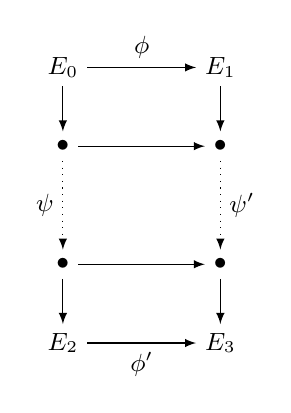
\begin{tikzpicture}
    \small
    \node (E0) at (0,0) {$E_0$};
    \node (E1) at (2,0) {$E_1$};
    \node (Ee0) at (0,-1) {$\bullet$};
    \node (Eo0) at (2,-1) {$\bullet$};
    \node (Ee1) at (0,-2.5) {$\bullet$};
    \node (Eo1) at (2,-2.5) {$\bullet$};
    \node (E2) at (0,-3.5) {$E_2$};
    \node (E3) at (2,-3.5) {$E_3$};

    \draw[-latex]
    (E0) edge node[above] {$\phi$} (E1)
    (Ee0) edge (Eo0)
    (Ee1) edge (Eo1)
    (E2) edge node[below] {$\phi'$} (E3)
    (E0) edge (Ee0)
    (E1) edge (Eo0)
    (Ee1) edge (E2)
    (Eo1) edge (E3);
    \draw[dotted,-latex]
    (Ee0) edge node[left] {$\psi$} (Ee1)
    (Eo0) edge node[right] {$\psi'$} (Eo1);
  \end{tikzpicture}
\end{equation*}
\caption{An SIDH ladder.} \label{fig:ladder}
\end{figure}

Additionally, one may glue SIDH squares both vertically and
horizontally, thus freeing the protocol from the constraint of having
the isogeny degrees divide $p+1$.


\subsection{SIDH signatures}

The Fiat-Shamir heuristic can be used to make sigma protocols non-interactive.
%From the point of view of signatures it is most efficient to stick with the simplest protocols.
The basic DFJP protocol from Section~\ref{sec:DFJP} has been used to construct a signature scheme in Yoo et al~\cite{YAJJS17} and~\cite{GPS20}, based on the hardness of DSSP and SIDH key exchange.
%the relation \R[isog]. \LDF{\R[SIDH]?}
These schemes are no longer secure, due to the attacks on SIDH, but it is fairly straightforward to construct secure signatures based on any of the protocols with ternary challenges above.



%\subsection{Other approaches}
%
%k-SIDH?
%
%\LDF{Hmmm, not really a PoK, is it?}
%\SG{Agree. Delete this}


\subsection{Questions and perspectives}

We now discuss some of the limitations of the protocols above.

\paragraph{Efficiency.}
A 3-special sound protocol comes at a cost: to achieve soundness error of $2^{-\lambda}$, one needs $\lambda/(\log_2(3)-1)$ iterations, each iteration computing one or more SIDH squares.
A major open problem is whether there exist protocols for any of these relations with small soundness error, possibly exponentially small.
SQISign, presented in Section~\ref{sec:SQIsign}, will provide a beginning of an answer for the relation $\R[isog]$.

\paragraph{Statistical ZK for \R[deg].}
Currently, there appears to be a tension between soundness and
zero-knowledge for \R[deg]: the ``flipping the SIDH square'' technique
of Section~\ref{sec:R-deg} is incompatible with the ``SIDH ladders''
of Section~\ref{sec:from-comp-stat}.  Indeed, in an SIDH ladder the
$D$-torsion is not anymore defined over the base field, and it is thus
not possible to define the torsion bases $(P_2,Q_2),(P_3,Q_3)$ used to
prove special soundness for \R[deg].

It is an interesting question to find alternative representations for
$D$-torsion bases that are compatible with SIDH ladders.
%\LDF{Actually, I think I know how to do this, but I'm not sure I want to do it!}

\paragraph{ZK for \R[isog]}
All the protocols we presented so far appear to leak $\deg(\phi)$ to
the verifier when responding with the isogeny $\phi'$ parallel to
$\phi$. It seems thus difficult to make them zero-knowledge for
\R[isog], rather than \R[deg].

%Is is equally interesting to find a zero-knowledge protocol, computationally or statistically, for the \R[isog] relation in the case where the endomorphism ring is not known.




\section{GPS and SQISign\label{sec:GPSandSQIsign}}

The GPS and SQISign protocols we describe in this section work with the full supersingular isogeny graph (unlike the CSIDH-based protocols of Section~\ref{sec:CSIDH} which only consider curves defined over $\mathbb{F}_p$), and use the quaternion algorithms described in Section~\ref{sec:KLPT} to design a GMW-like protocol which does not rely on a SIDH diagram. 
The GPS protocol provides steps towards a general solution to proving the relation $\R[isog]$.
In particular, the GPS protocol achieves statistical ZK, and no auxiliary points or other information are needed to obtain zero-knowledge.



\subsection{GPS sigma protocol} \label{sec:GPSproof}



%This section explains how to take the naive protocol from Section~\ref{sec:simple} and make it secure. The key idea is a method to ``re-randomise'' $\rho = \psi \circ \phi$, so that the response to the challenge is a uniformly sampled isogeny from $E_0$ to $E_2$.
%This conjecturally gives statistical ZK. \CP{why ``conjecturally''?}

The GPS protocol, due to Galbraith, Petit, and Silva~\cite{GPS20},  heavily uses the ideas of Section~\ref{sec:KLPT}. In particular, we assume that $E_0$ is a special supersingular curve such as $y^2 = x^3 + x$.
We wish to prove knowledge of an isogeny $\phi : E_0 \to E_1$, and will use properties of $\End(E_0)$.
So our protocol proves $\R[isog]$ for any field, but in the special case where $E_0$ is a curve with known endomorphism ring.

To prove knowledge of an isogeny between two ``arbitrary'' curves $E'$ and $E''$ one can apply this protocol if one knows an isogeny from $E_0$ to $E'$ (and hence one can construct an isogeny from $E_0$ to $E''$).
However, if $E'$ and $E''$ are curves whose endomorphism ring is not known to the prover then the methods of this section cannot be applied.

The sigma protocol is as follows.
First, fix parameters $B$, $N_1$, $N_2$ such that $N_k =\prod_i\ell_{k,i}^{e_{k,i}}$, where $\ell_{k,i}^{e_{k,i}}<B$, $\gcd(N_1,N_2)=1$, $\log(N_2) > \tfrac{7}{2} \log(p)$, and for each $k \in \{1,2\}$
\[
  \prod_i\left(\frac{2\sqrt{\ell_{k,i}}}{\ell_{k,i}+1}\right)^{e_{k,i}}<(p^{1+\epsilon})^{-1}. 
\]
This last formula is needed for uniform mixing of random walks in the isogeny graph.
We let $I$ be the left $\OO_0$-ideal corresponding to the secret isogeny $\phi : E_0 \to E_1$.

To construct the commitment $\com$, perform a random isogeny walk of degree $N_1$ from the curve $E_1$ to a curve $E_2$ and set $\com = j(E_2)$.
The isogeny $\psi : E_1 \to E_2$ can be represented in many ways (e.g., kernel points of order $\ell_i^{e_i}$ or a sequence of $j$-invariants).
Let $J$ be the left-$\End(E_1)$-ideal corresponding to $\psi$.
Let the challenge be $\chall \in \{0,1\}$.
When $\chall=0$ respond with $\psi$.
When $\chall=1$ the KLPT algorithm is needed. We compute the ideal $IJ$, which corresponds to $\psi \circ \phi$.
Then run KLPT to get an equivalent $\OO_0$-ideal $J'$ of norm $N_2$. The response is the isogeny $\psi' : E_0 \to E_2$ corresponding to $J'$.
The verifier checks that the response is an isogeny from $E_{1-\chall}$ to $E_2$.
The protocol is repeated until the verifier is convinced.

The special soundness of the protocol is easy to prove. Given valid responses $\psi'$ and $\rho$ to the challenges 0 and 1 for the same commitment, the extractor can compute an isogeny $\rho \circ \hat\psi'$ from $E_0$ to $E_1$. Note that this isogeny is a priori not the same one used by the prover to create the responses, but this is irrelevant to special soundness\footnote{Additionally, both isogenies can in fact be mapped to the same ``canonical'' one (for example, using LLL to compute a minimal norm ideal in the ideal class, followed if needed by some deterministic version of KLPT to get a powersmooth norm ideal).}.


The three key requirements for this to be zero-knowledge and practical are that:
\begin{enumerate}
    \item $E_2$ is close to uniformly distributed in the isogeny graph.
    \item The isogeny $\psi'$ is independent of $\phi$.
    \item The isogenies $\psi$ and $\psi'$ in the response have a compact representation and can be computed efficiently.
\end{enumerate}
The first two properties are needed for zero-knowledge. 
The simulator, who knows the challenge but who does not know $\phi$ or $I$, will behave as in the honest protocol for the case $\chall=0$, but when $\chall=1$ will take a random isogeny from $E_0$ to $E_2$ and then run KLPT to get an ideal $J'$ as in the real protocol. 
It is necessary that the curves $E_2$ generated by the simulator when $\chall=1$ are distributed close to identically as in the original protocol. This is the purpose of the first requirement.
It is also necessary that the isogenies $\psi'$ are distributed identically in both cases.
We refer to~\cite{GPS20} for the details.


As the protocol uses one-bit challenges, it must be repeated $\lambda$ times to obtain a scheme with $2^{-\lambda}$ soundness error.
The protocol can be made non-interactive and used as a signature scheme by the Fiat-Shamir transform. While polynomial time in theory, the resulting signature scheme is considered impractical.
%, and it has never been implemented.


%This is still using single bit challenges.
%In some cases (depending on the witness $\phi$) we might be able to apply the ideas of SQI-Sign. \CP{I don't get the last sentence}




\subsection{SQISign \label{sec:SQIsign}}

A key source of inefficiency in GPS signatures (and other signatures based on isogenies) is the need to repeat the zero-knowledge protocol multiple times to reduce the soundness error. This comes from the fact that the protocol has single bit challenges.


To increase the challenge space, the SQISign protocol by De Feo, Kohel, Leroux, Petit, and Wesolowski~\cite{DFKLPW20} modifies the basic GMW-based protocol as follows. Given a secret isogeny $\phi:E_0\rightarrow E_1$, the prover first computes a random isogeny $\psi:E_0\rightarrow E_2$ and commits to $E_2$. Then instead of challenging the prover with a single bit, the verifier computes and sends a third random isogeny $\varphi:E_2\rightarrow E_3$, sends it to the prover, and challenges the prover to compute an isogeny $\sigma:E_1\rightarrow E_3$ (see Figure~\ref{fig:sqisign}).

\begin{figure}[h!]
    
  
\begin{center}
   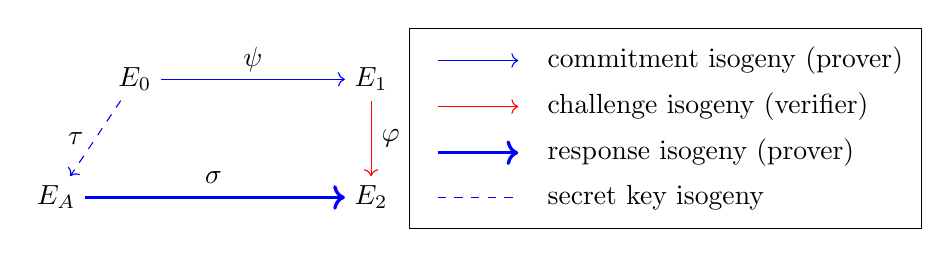
\begin{tikzpicture}
    \node (E0) at (1,2.5) {$E_0$};
    \node (E1) at (4,2.5) {$E_1$};
    \node (E2) at (4,1) {$E_2$};
    \node (EA) at (0,1) {$E_A$};
    \node (A) at (0.25,1.75) {$\tau$};
    \node (B) at (2.5,2.75) {$\psi$};
    \node (A) at (4.25,1.75) {$\varphi$};
    \node (B) at (2,1.25) {$\sigma$};
    % \draw [->] (E) -- (E1);
    \draw [blue,very thick] [->] (EA) -- (E2);
    \draw [red] [->] (E1) to (E2);
    \draw [blue,dashed] [->] (E0) to (EA);
    \draw [blue] [->] (E0) to (E1);
    \matrix [draw, right] at (current bounding box.east) {
\node[] (l1) {}; \node (l2) [right of = l1, node distance=0.5in,label=right: commitment isogeny (prover)] {}; \draw [blue] [->] (l1) -- (l2); \\
\node[] (l3) {}; \node (l4) [right of = l3, node distance=0.5in,label=right:challenge isogeny (verifier)] {}; \draw [red] [->] (l3) -- (l4); \\
\node[] (l1) {}; \node (l2) [right of = l1, node distance=0.5in,label=right: response isogeny (prover)] {}; \draw [blue,very thick] [->] (l1) -- (l2); \\
\node[] (l1) {}; \node (l2) [right of = l1, node distance=0.5in,label=right: secret key isogeny] {}; \draw  [dashed,blue] [-] (l1) -- (l2); \\
};
\end{tikzpicture}
\end{center} \caption{A picture of SQIsign's identification protocol~\cite{DFKLPW20}}   \label{fig:sqisign} \end{figure}

%\WB{reviewer says: "a commutative diagram to accompany the second paragraph of section 6.2 would be a worthy addition imo"}

A naive version of this protocol is not secure: A dishonest prover could compute the commitment by computing a random isogeny $\psi'$ from $E_1$. Call $E_2$ the image curve. Since the verifier sends an isogeny $\varphi$ the prover can respond with $\varphi \circ \psi' : E_1 \to E_3$.
The way to prevent this is for the verifier to check that $\hat{\varphi} \circ \sigma$ has cyclic kernel; we refer to~\cite{DFKLPW20} for the details.
The protocol also imposes conditions on the isogeny $\phi:E_0\rightarrow E_1$, namely that $E_0$ has known endomorphism ring and that $\phi$ has ``medium'' prime degree.
Finally, the protocol is only computationally ZK based on an ad hoc assumption.
Hence SQISign is currently far from a general solution to the relation $\R[isog]$.

Special soundness relies on the problem of computing an endomorphism of $E_1$, a problem equivalent to computing an isogeny between two random supersingular  curves~\cite{GPS20,Reductions18,Wes22}.


%
Indeed, given two valid responses to two challenges for the same commitment, an extractor can compose both challenges and responses in an appropriate way to compute an endomorphism of $E_1$ (see~\cite{DFKLPW20}).\footnote{A similar approach in the case of graph isomorphism would provide the extractor with an automorphism of one graph. This does not immediately solve the graph isomorphism problem.}
%\CP{but  can maybe be used to accelerate Babai's algorithm?}}.

The astute reader will have noticed that computing $\sigma$ now requires to re-randomize an isogeny between two random supersingular curves, whereas the tools described in Section~\ref{sec:KLPT} assumed one of the curves was ``special'', i.e. with known and very special endomorphism ring. One can trivially generalize these tools to the general case (in fact this was already done in~\cite{KLPT}), but in a way that, used in the above signature scheme, will always leak the secret (the isogeny $\sigma$ will always go through the curve $E_0$). 
%
The key contribution in~\cite{DFKLPW20} is a new generalization of the KLPT algorithm which conjecturally avoids this problem. 

SQISign signatures are an order of magnitude smaller than all other post-quantum isogeny-based signature schemes in the signature-plus-public-key metric. Key generation and verification time are reasonable (at 0.6s and 50ms respectively) but signing takes 2.5s, mostly because of the conversions between isogenies and ideals (which are polynomial time but slow in practice).
%
An improved version of the protocol obtained a more than two-fold speedup on signing time~\cite{SQIsign2.0}.
%
It is an open question whether SQISign can be fast enough for many applications. 

Further work should aim at improving the signing time, but also to address some outstanding security concerns:
\begin{itemize}
    \item SQISign is not known to be secure in the quantum oracle model. This is because the sigma protocol does not have any of the properties that allow proving the security of Fiat-Shamir signatures in this model~\cite{KLS18}. Possible solutions include switching to the Unruh transform~\cite{Unruh15} (at some efficiency cost) or developing an ad hoc proof.
    \item The SQISign security proof does not provide an extractor that outputs an isogeny from $E_0$ to $E_1$. So it is not technically a proof of knowledge for $\R[isog]$. 
    However, the extractor does return a ``random'' endomorphism on $E_1$.
    
    Heuristically, $O(1)$ independent endomorphisms should generate the whole endomorphism ring, and one can build~\cite{EHLMP20} a $k$-special sound extractor that computes the whole endomorphism ring (for $k=O(1)$). Proving this formally remains an open problem.
    Once $\End(E_1)$ is known then an isogeny from $E_0$ to $E_1$ can be computed~\cite{Wes22}.
    %
    \item Some issues with the zero-knowledge of SQISign were pointed out in~\cite{SQIsign2.0}, and tweaks to the algorithms to avoid the issue are provided.
    \item The security definition for computational honest verifier zero-knowledge in Definition~\ref{def:sigmaprot} allows the distinguisher to be provided with a witness, but the arguments for the computational honest verifier zero-knowledge property in~\cite{DFKLPW20} do not apply in this case. Indeed with a witness one can easily distinguish between the response isogeny and a random isogeny of the same degree between the same two curves (as a quick study of~\cite[Figure 3]{DFKLPW20} shows). One approach to solve this problem could be to randomize the output of the \emph{EquivalentPrimeIdeal} and/or the particular secret isogeny $\tau$ used in the generalized KLPT algorithm~\cite{DFKLPW20}. However, both approaches will increase the norm of the ideal that is output by this algorithm, and hence they will further slow down signature generation. We also leave the security analysis of these approaches to further work.
\end{itemize}








\section{Conclusion and open problems\label{sec:conclusion}}

We have explained that proving knowledge of an isogeny is an important problem with several strong motivations in post-quantum cryptography.
%
We have given a number of sigma protocols for different relations and contexts. Generally the case of group actions is simpler than the more general isogeny problems.
%and the SIDH problems. The SIDH case is quite complicated due to the necessity to work with auxiliary points.

One of the biggest open problems in this area is to develop more efficient protocols by lowering the soundness error.
In the CSIDH setting we have signature schemes that have improved soundness error, but those approaches do not solve the problem for the original relation $\R[isog]$ we are interested in.
%In SIDH we do not have any protocol with soundness error strictly less than $ 1/2$.
The only example of a protocol with negligible soundness error for a single round is SQISign.
Any progress on reducing the soundness error would have major implications on the efficiency of isogeny signatures.

Another major open problem is to design a protocol for the relation $\R[isog]$ that can be applied when $\End(E)$ is not known and that does not leak the degree of the witness. The GPS scheme~\cite{GPS20} only works when $\End(E)$ is known, while SQISign is currently not a proof of knowledge.


Further open questions that we have discussed in the paper include:
How effective are general tools for ZK proofs when applied to isogeny problems?
Can zero-knowledge of SQISign (or a variant of it) be proved based on more standard assumptions?
Are there ways to get signatures with a tight reduction to (relatively) standard assumptions?


\bibliographystyle{alpha}
\bibliography{isogeny}

\end{document}
